\documentclass[type=master]{thuthesis}
% 选项:
%   type=[bachelor|master|doctor|postdoctor], % 必选
%   secret,                                   % 可选
%   pifootnote,                               % 可选(建议打开)
%   openany|openright,                        % 可选,基本不用
%   arial,                                    % 可选,基本不用
%   arialtoc,                                 % 可选,基本不用
%   arialtitle                                % 可选,基本不用

% 所有其它可能用到的包都统一放到这里了,可以根据自己的实际添加或者删除。
\usepackage{thuthesis}
\usepackage{graphicx}
\usepackage{amssymb}
\usepackage{amsmath}
\usepackage{listings}
\usepackage{algorithm}
\usepackage{algorithmic}
\usepackage{multirow}
\usepackage{float}
%\usepackage[caption = false]{subfig}
\DeclareMathOperator*{\argmax}{arg max}
\DeclareMathOperator*{\argmin}{arg min}
%\newtheorem{theorem}{Theorem}[section]
%\newtheorem{proposition}[theorem]{Proposition}


% 定义所有的图片文件在 figures 子目录下
\graphicspath{{figure/}}

% 可以在这里修改配置文件中的定义。导言区可以使用中文。
% \def\myname{薛瑞尼}

\begin{document}

%%% 封面部分
\frontmatter
\thusetup{
  %******************************
  % 注意:
  %   1. 配置里面不要出现空行
  %   2. 不需要的配置信息可以删除
  %******************************
  %
  %=====
  % 秘级
  %=====
  secretlevel={秘密},
  secretyear={10},
  %
  %=========
  % 中文信息
  %=========
  ctitle={ASPCA 一种基于PCA异常空间稀疏化的异常诊断方法},
  cdegree={工学硕士},
  cdepartment={计算机科学与技术系},
  cmajor={计算机科学与技术},
  cauthor={宾行言},
  csupervisor={赵颖副教授},
  % 日期自动使用当前时间,若需指定按如下方式修改:
  % cdate={超新星纪元},
  %
  % 博士后专有部分
  %
  %=========
  % 英文信息
  %=========
  etitle={Abnormal Subspace Sparse PCA for Anomaly Detection and Interpretation},
  % 这块比较复杂,需要分情况讨论:
  % 1. 学术型硕士
  %    edegree:必须为Master of Arts或Master of Science(注意大小写)
  %             “哲学、文学、历史学、法学、教育学、艺术学门类,公共管理学科
  %              填写Master of Arts,其它填写Master of Science”
  %    emajor:“获得一级学科授权的学科填写一级学科名称,其它填写二级学科名称”
  % 2. 专业型硕士
  %    edegree:“填写专业学位英文名称全称”
  %    emajor:“工程硕士填写工程领域,其它专业学位不填写此项”
  % 3. 学术型博士
  %    edegree:Doctor of Philosophy(注意大小写)
  %    emajor:“获得一级学科授权的学科填写一级学科名称,其它填写二级学科名称”
  % 4. 专业型博士
  %    edegree:“填写专业学位英文名称全称”
  %    emajor:不填写此项
  edegree={Master of Science},
  emajor={Computer Science and Technology},
  eauthor={Bin Xingyan},
  esupervisor={Associate Professor Zhao Ying},
  % 日期自动生成,若需指定按如下方式修改:
  % edate={December, 2005}
  %
  % 关键词用“英文逗号”分割
  ckeywords={机器学习, 异常检测, 异常诊断, PCA, 稀疏},
  ekeywords={machine learning, anomaly detection, anomaly analysis, PCA, sparsity}
}

% 定义中英文摘要和关键字
\begin{cabstract}
  主成分分析(PCA)在被运用到异常检测中时,其主要缺点在于其可解释性。在这篇文章中,所介绍的ASPCA模型是一个在可解释性方面有了很大改善的基于PCA的改进模型。模型核心机理是通过构建具有系数稀疏与正交特点的主成分来描述异常空间。
  
  通过在一个模拟数据集以及两个真实数据集上所进行的实验表面,该模型在异常检测精度方面,效果与原始的PCA方法近似,并且可以针对每一个检测出来的异常进行单独分析。

\end{cabstract}

% 如果习惯关键字跟在摘要文字后面,可以用直接命令来设置,如下:
% \ckeywords{\TeX, \LaTeX, CJK, 模板, 论文}

\begin{eabstract}
	The main shortage of principle component analysis (PCA) based anomaly detection models is their interpretability. In this paper, our goal is to propose an interpretable PCA- based model for anomaly detection and interpretation. The propose ASPCA model constructs principal components with sparse and orthogonal loading vectors to represent the abnormal subspace, and uses them to interpret detected anomalies. Our experiments on a synthetic dataset and two real world datasets showed that the proposed ASPCA models achieved comparable detection accuracies as the PCA model, and can provide interpretations for individual anomalies.
  
\end{eabstract}

% \ekeywords{\TeX, \LaTeX, CJK, template, thesis}

% 如果使用授权说明扫描页,将可选参数中指定为扫描得到的 PDF 文件名,例如:
% \makecover[scan-auth.pdf]
\makecover

%% 目录
\tableofcontents

%% 符号对照表
\begin{denotation}[3cm]
\item[PCA] Principle Component Analysis 主成分分析
\item[cluster] 集群
\item[Itanium] 安腾
\item[SMP] 对称多处理
\item[API] 应用程序编程接口
\item[PI] 聚酰亚胺
\item[MPI] 聚酰亚胺模型化合物,N-苯基邻苯酰亚胺
\item[PBI] 聚苯并咪唑
\item[MPBI] 聚苯并咪唑模型化合物,N-苯基苯并咪唑
\item[PY] 聚吡咙
\item[PMDA-BDA]	均苯四酸二酐与联苯四胺合成的聚吡咙薄膜
\item[$\Delta G$] 活化自由能 (Activation Free Energy)
\item[$\chi$] 传输系数 (Transmission Coefficient)
\item[$E$] 能量
\item[$m$] 质量
\item[$c$] 光速
\item[$P$] 概率
\item[$T$] 时间
\item[$v$] 速度
\item[劝学] 君子曰:学不可以已。青,取之于蓝,而青于蓝;冰,水为之,而寒于水。木
  直中绳。輮以为轮,其曲中规。虽有槁暴,不复挺者,輮使之然也。故木受绳则直,金就
  砺则利,君子博学而日参省乎己,则知明而行无过矣。吾尝终日而思矣,不如须臾之所学
  也;吾尝跂而望矣,不如登高之博见也。登高而招,臂非加长也,而见者远;顺风而呼,
  声非加疾也,而闻者彰。假舆马者,非利足也,而致千里;假舟楫者,非能水也,而绝江
  河,君子生非异也,善假于物也。积土成山,风雨兴焉;积水成渊,蛟龙生焉;积善成德,
  而神明自得,圣心备焉。故不积跬步,无以至千里;不积小流,无以成江海。骐骥一跃,
  不能十步;驽马十驾,功在不舍。锲而舍之,朽木不折;锲而不舍,金石可镂。蚓无爪牙
  之利,筋骨之强,上食埃土,下饮黄泉,用心一也。蟹六跪而二螯,非蛇鳝之穴无可寄托
  者,用心躁也。—— 荀况
\end{denotation}



%%% 正文部分
\mainmatter
\chapter{绪论}
\label{cha:intro}
PCA是一种常用的基于统计的异常检测模型。很多研究者尝试将该方法运用于网络流量分析与攻击检测\cite{Anomaly-Survey-09,XuWeiGoogle,Lakhina-2005-sigcomm,jiang2013family},但该方法不仅仅只是学术领域的尝试,在生产系统中,例如美国最大的版权电视节目网站Netflix就在使用PCA算法作为他们的安全检测算法\cite{netflix-outlier}。除了计算机领域,PCA模型还可以被运用在金融领域\cite{jiang2013family}以及航天领域\cite{dutta2007distributed}。在微软机器学习云服务中,对于异常检测它推荐了两种算法,对于特征数量比较有限的场景,微软的推荐就是基于PCA的异常检测方法\cite{microsoft-cheatsheet}。

在实际应用中,如果在异常检测时,能够阐释其判断的依据,则能够帮助解决这些异常。例如航天系统的某个异常,如果可以描述出具体的判断依据,则可以更快的进行问题的排查,更快的恢复系统工作。例如对于网络入侵的检测,如果能给出判断依据,则可以由系统管理员对系统的相应环节进行更好的安全加固。我们把这种可以对于每一个检测出的异常都能够给出人所能解读其依据的能力,称为{\bf 异常解释(anomaly interpretation)}。一个具有异常解释能力的异常检测系统将会更具有实用价值。

然而,传统的基于PCA模型的异常检测模型不能很好的进行异常解释\cite{XuWei-SOSP,PCA-Sensitivity}。

PCA分辨异常依据的是某个数据点不符合数据集主流的统计规律。而PCA所挖掘的主流统计规律是在原始数据空间中,存在一个低维的子空间能够容纳数据的主要波动。当数据点不能完全被这样的一个低维子空间所容纳时,模型判断它为异常。由于最终指示数据点是否为异常的指标与原始数据之间存在很多步骤,并且由于对低维子空间的描述非常复杂,导致中间处理步骤的计算也是非常复杂的,因此这样的计算过程很难进行解释。利用PCA进行异常检测的方法被人视作是一种黑箱方法\cite{XuWei-SOSP}。

人们为了解决这个问题,从不同的方向进行了尝试。\cite{XuWei-SOSP} 在通过用PCA进行异常检测后,增加了一个新的步骤,利用决策树模型来解释检测出的异常,决策树模型具有很好的可解释性。但是,这种间接的解释方式,不能真正解释PCA异常检测方法判断异常的原因\cite{PCA-Sensitivity}。另一个工作\cite{jiang2013family}提出了联合稀疏化PCA(JSPCA)的新模型,该模型提出用一个新的子空间去近似描述数据空间中不能被代表主流规律的子空间所接受的部分,这个新空间将只涉及到少数原本空间的特征维度。这种方法定位了哪些特征维度会与检测数据所有的异常点相关。但对于每个单独的异常记录,尤其是完全不同的异常记录,该模型却只能给出相同的模糊指示。总之,现有方法无法准确地,直接地给出每个异常记录被判断为异常的依据,无法进行异常解释。

我们的目的是设计一种基于PCA的改进模型,使得它能够同时进行异常检测与异常解释。模型同样是尝试获取一个新的子空间来描述数据中不能被主流规律子空间所接受的部分。这样的子空间具有以下特点:与主流规律子空间正交,描述该子空间所用的基向量具有正交和稀疏的性质。我们将这种可解释的异常检测模型称为{\bf ASPCA}(Anomaly subspace Sparse PCA)即异常子空间稀疏化PCA。

本文主要工作有,首先,提出了ASPCA模型的两种计算方式。第一种是按照PCA求解一般惯例地,从最主要的主成分开始进行提取,然后再提取剩余的主成分,即先提取体现主流变化的子空间,它所剩余的子空间构成了我们所要的分析异常的子空间;第二种方式与之相反,将从变化量(Variance)最小的主成分开始提取,即直接获取我们用来分析异常的子空间。其中,第二种方式将会在异常子空间下获取更好的稀疏性质。本文提出的ASPCA模型是第一个基于PCA模型,且能进行单个异常记录的检测解释能力的模型。其次,我们通过半正定规划(SDP,Semidefinite programming)对提出的模型进行一定程度的放松之后进行优化求解,并且在逐个求出异常子空间的主成分后,还对该子空间以稀疏性为目标进行了全局优化,尝试获得更好的稀疏性质。

本文中的实验通过一个人工数据以及两个真实数据展示了ASPCA模型所能取得的与PCA在异常检测方面相似的表现,以及对逐个检测出的异常记录进行解释的能力。

本文之后的章节如下:第二章介绍相关工作,第三章介绍我们所提出的ASPCA模型,第四章介绍优化算法,第五章介绍实验,最后在第六章进行一些总结。



\chapter{相关工作}
PCA方法最为人所知的用法,是用于特征压缩\cite{jolliffe2002principal},通过PCA对数据的挖掘,可以得到更少的新的特征来描述整个数据集的变化。而同时,也有很多工作将其作为一种异常检测方法\cite{dunia1997multi,Anomaly-Survey-09}。Wei Xu 等人将该技术用于分析日志,并且将其运用在一个游戏服务器上,还利用该方法检测出了Hadoop File System(HDFS)的一些问题\cite{XuWei-SOSP}。该工作还被运用在了Google的生产系统中\cite{XuWeiGoogle}。Ryohei Fujimaki 等人将 kernel PCA 用在了宇宙飞船的异常检测问题上 \cite{kernelPCA-Space}。
还有很多研究者将PCA技术用在了网络入侵检测上\cite{Lakhina-2005-sigcomm,Lakhina-2004-sigcomm,jiang2013family,PCA-KDD99-2006}。Shyu, M.L. 等人利用大成分(数据变化大的部分)以及小成分(数据变化小的部分,也就是本工作所定义的异常子空间)形成 Mahalanobis距离,取代一般所用的小成分空间的欧氏距离,并且采用鲁棒PCA来提升无监督异常检测的表现\cite{shyu2003novel}。Anukool Lakhina 等人将PCA模型运用在了网络洪流检测问题当中,所分析的数据是关于每一个源头-目的地二元组与时间的矩阵\cite{Lakhina-2005-sigcomm,Lakhina-2004-sigcomm}。首先,他们主要是分析通信的流量大小\cite{Lakhina-2004-sigcomm},之后他们将通信流量的熵也作为描述二元组的另一个特征引入进来,形成多子空间的PCA检测\cite{Lakhina-2005-sigcomm}。Ling Huang 等人还尝试设计了一种在线PCA监测模型,模型考虑了可扩展性以及分布式布置下的通信效率\cite{huang2006network,INFOCOM-Distributed-PCA}。

当将PCA作为一种特征压缩工具时,其主要缺点在于糟糕的可解释性。Ian Jolliffe 等人引入了稀疏PCA的概念,在这种概念下,对提取出的特征参数向量进行了稀疏性方面的限制\cite{SPCA-2003}。自此,产生了很多求解稀疏PCA问题的算法,例如 \cite{SPCA-2006} 和 \cite{SPCA-SDP}。Hui zou 等人将稀疏PCA问题转化为了一个带elastic net正规项的回归问题,该问题可以通过交替最小化(alternating minimization)的算法进行求解\cite{SPCA-2006}。Alexandre d'Aspremont 等人通过对原问题的一些条件的放松,提出了通过半正定规划(SDP)求解稀疏PCA问题,该方法从大到小逐个求解主成分\cite{SPCA-SDP}。

当将PCA作为一种异常检测工具时,糟糕的可解释性同样是它的缺点 \cite{PCA-Sensitivity,XuWei-SOSP}。Ruoyi Jiang 等人受到稀疏PCA启发,引入了连接稀疏PCA的方法来解决异常定位问题\cite{jiang2011JSPCA,jiang2013family}。他们的工作采用的是交替最小化的框架\cite{SPCA-2006}来解决他们所提出的优化问题。 Wei Xu 等人也尝试了解决PCA异常检测可解释性查的问题。他们讲检测模型所得到的异常记录标记上标签,将其与正常记录作为训练数据输入到决策树模型。决策树模型是一个具有很好的可解释性的模型,但正如我们之后的实验结果所表现的那样,这种方案所找到的解释可能与PCA模型相悖,因为他体现的并不是PCA模型本身的依据,而是PCA检测结果的统计表现,也就是一种“事后诸葛亮”的分析,并不能反映检测本身的思路。

\chapter{PCA与异常检测}
\subsection{符号}
粗体大写字母表示的是矩阵,类似于${\bf X}$。粗体小写字母表示列向量,类似于${\bf x}$。希腊字母表示系数,类似于 $\lambda,\mu$。 $||{\bf X}||_F$ 表示矩阵 ${\bf X}$ 的F-范数,而 $||{\bf X}||_{1,1}$ 表示 ${\bf X}$ 的 $L_{1,1}$ 范数。也即 $||{\bf X}||_{1,1} = {\bf 1}|{\bf X}|{\bf 1}^T$。

数据集表示为一个 $n \times p$ 的数据矩阵 ${\bf D}$,其中每一个行向量表示一个$p$维的记录,而每一个列向量则是一个特征向量。${\bf A} = {\bf D}^T{\bf D}$是数据矩阵${\bf D}$的协方差矩阵。$Tr({\bf A})$ 表示矩阵 ${\bf A}$的迹。而$Card({\bf A})$ 表示矩阵${\bf A}$的势,即矩阵的非零元素个数。${\bf I}$是一个单位矩阵。$\mathbb{S}^p$ 是所有所有$p \times p$维矩阵即$\mathbb{R}^{p \times p}$的对称半正定矩阵构成的子集。

\subsection{PCA异常检测模型}
主成分分析(PCA)通常被用于进行特征压缩,即对于一个数据矩阵,他可以提取出体现了数据主要变化的一组特征,而这组特征是由数据原本的特征线性组合得到的。假设给定一个$p$维的数据集,即有$p$个特征,数据存在的$p$维欧氏空间命名为空间A,空间通过它的$p$个基向量来进行描述。虽然一个空间可以用无数组基向量来描述,但一般都通过最简洁的正交基进行描述,对于原始空间而言,最好的就是各个特征方向上的基向量,他们整体组成一个单位矩阵。而PCA所发掘的新的特征实际上是原始空间的一个子空间,在这一个子空间内,体现了数据的主要变化,即数据在这个子空间中总的方差最大,这个子空间在作为特征压缩应用时,我们称其为主要子空间。

使用PCA来进行异常检测的主要思路在于,对于整体而言主要变化同时体现的也是主流的变化,即大多数的数据点都能够很好的用降维的特征来进行描述,对这些个体而言,它们在PCA得到的主要子空间内的投影向量与自身基本相符。但同时还存在一些数据点,如果用降维得到的特征来进行描述将会丢失很多信息,即它们在PCA得到的主要子空间内的投影向量与自身差异较大。

举例而言,用太阳系八大行星加上冥王星的三维运行轨迹点作为分析数据集,我们将会发现,数据的主要变化都在黄道平面上,因此,实际上我们可以只用黄道平面上的坐标就足够描述行星运动。八大行星的运动都能很好的用黄道平面坐标描述,但是冥王星在黄道平面上的投影向量与自身实际位置向量常常会有很大的偏差,因此,我们可以判别冥王星的运动不符合主流。而事实上,其运动不符合主流也是冥王星被排除出太阳系大行星行列的主要原因之一。

之前提到,数据的主要变化体现了数据的主流变化,但其实这个判断在一些情况下并不准确。因为有的时候非主流的变化可能会对整体变化造成非常大的影响,这在实际生活中并不鲜见。在统计分析中,摒除掉非主流样例对把握主流特征的干扰被称为鲁棒统计分析,PCA同样也有一部分分支为鲁棒PCA分析(Robust PCA),并且这一类分析也被运用到了异常检测当中。我们的工作没有讨论这一部分的延伸,但可以通过一些初步的处理来去除掉异常数据点的对主流规律的干扰,例如将一些数值明显超出正常范畴的数据点不纳入到PCA得到主要子空间的分析数据内。

另外,PCA异常检测得到的是数据中的非主流数据点,在实际生活中,非主流数据点未必是非正常数据点即异常数据点,主流并不是正常的同义词。但在非监督的统计分析当中,也只能检测得到非主流的信息,而大多数情况下,非主流和异常是存在大量重合的。

在异常检测任务中,我们将主要子空间称为正常子空间,而与之互补的子空间称为异常子空间。

PCA分析得到的是一系列构成新特征的系数向量以及数据依据系数向量所构成的${\bf 主成分}$。第一个主成分是数据集下,能够获取最大方差的特征方向上的投影值。随后的主成分则是与之前的主成分线性无关条件下所能获取的最大方差特征方向上的投影值。前$k$个主成分以及相应的系数向量构成了主要子空间,即正常子空间。其中系数向量即为空间的正交基。而剩余的主成分和系数向量则构成了异常子空间。

如前所述,判断一个数据点是否为异常的依据是该数据点向量与其在正常子空间下的投影向量的偏差\cite{PCA-Sensitivity}。用数学符号来表达即为:

定义 ${\bf V}_1=({\bf v}_1,\cdots,{\bf v}_k)$ 为靠前的$k$个主成分所处的正常子空间,${\bf v}_1,\cdots,{\bf v}_k$ 是各个主成分所对应的系数向量,系数向量互相垂直。而${\bf V}_2=({\bf v}_{k+1}, \cdots,$ ${\bf v}_p)$ 则是剩余的 $p-k$ 个主成分所处的异常子空间,同样是通过主成分所对应的系数向量 ${\bf v}_{k+1},\cdots,{\bf v}_p$ 作为基向量来构建该子空间。对于一个 $p$ 维的数据点 $y$,其自身与其在正常子空间下的投影向量的偏差 $\hat{{\bf y}}$ 可以表示为:

\begin{equation}
\hat{{\bf y}} = {\bf y}-{\bf V}_1{\bf V}_1^T{\bf y}.
\end{equation}

${\bf \hat{y}}$的平方长度被称为SPE(squared prediction error),即通过PCA来预测还原数据的误差。SPE是PCA模型用来判定数据点 ${\bf y}$ 是否异常的指标。SPE越大,则该数据点越可能是一个异常。实际使用中,会设置一个阈值来判断是否异常,阈值的大小由使用者从准确率以及回归率等方面进行权衡。

\subsection{异常解释}

而如何理解判定其为异常的依据,即数据点 ${\bf y}$ 哪些方面的表现使得他的与正常子空间下投影的偏差过大,即PCA模型异常检测的异常解释问题。虽然偏差向量 $\hat{{\bf y}}$ 的长度是检测异常的主要依据,但用 $\hat{{\bf y}}$ 向量本身的各个维度上的值来解释是没有意义的。因为这些维度上的值并不该数据点 ${\bf y}$ 原本特征维度上的数值有直接的对应关系\cite{PCA-Sensitivity},也就是说,这些值的来源很难解释。

正常子空间${\bf V}_1$下向量与投影的偏差$\hat{{\bf y}}$其实就是向量在正常空间的补空间即异常子空间 ${\bf V}_2$ 上的投影,即有:

\begin{equation}
\label{equation:yHat}
\begin{split}
\hat{\bf{y}} &= {\bf y}-{\bf V}_1{\bf V}_1^T{\bf y} \\
 & = {\bf V}_2{\bf V}_2^T{\bf y}.
\end{split}
\end{equation}

我们设定异常子空间 ${\bf V}_2=({\bf v}_{k+1}, \cdots, {\bf v}_p)$,其中 ${\bf v}_{k+1},\cdots,{\bf v}_p$ 是一组互相垂直的系数向量,由他们作为正交基来表示异常子空间。依据\ref{equation:yHat},可以得到SPE为:


\begin{equation}
\label{equation:SPE}
\begin{split}
SPE &= \hat{{\bf y}}^T\hat{{\bf y}} = {\bf y}^T{\bf V}_2 {\bf V}_2^T {\bf V}_2 {\bf V}_2^T {\bf y}\\
       & = ({\bf y}^T{\bf V}_2)({\bf V}_2^T {\bf V}_2)({\bf V}_2^T {\bf y})\\
       & = ({\bf V}_2^T {\bf y})^T({\bf V}_2^T {\bf y})\\
       & = \sum_{i=k+1}^{p}({\bf v}_i^T {\bf y})^2.
\end{split}
\end{equation}


\begin{figure}
	\centering
	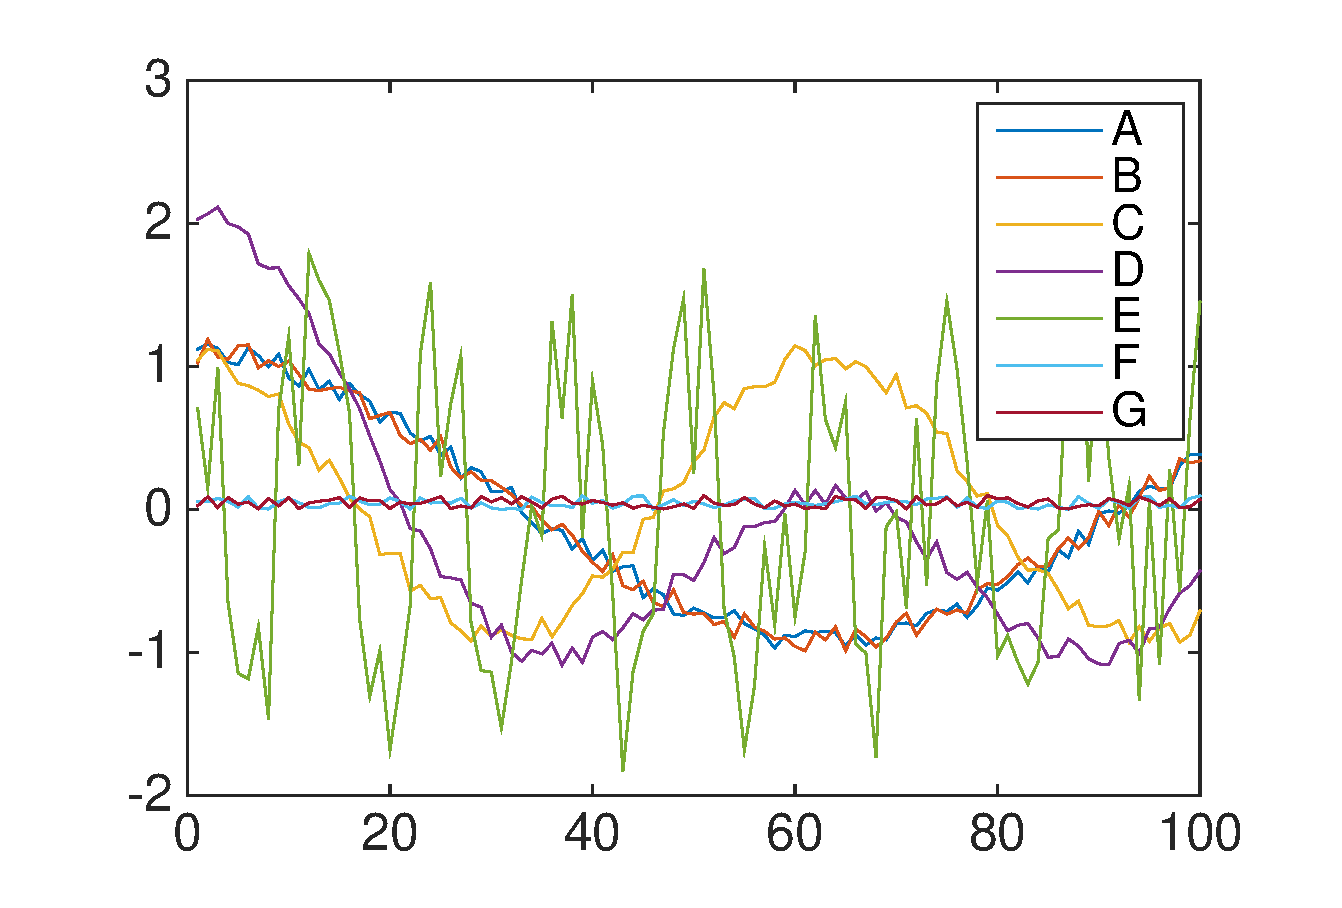
\includegraphics[width=80mm]{figure/lines/synthesized_data}
	\label{fig:synthesized_data}
	\caption{合成数据中的正常样例}
\end{figure}


\begin{figure}
\begin{minipage}{0.48\textwidth}
\centering
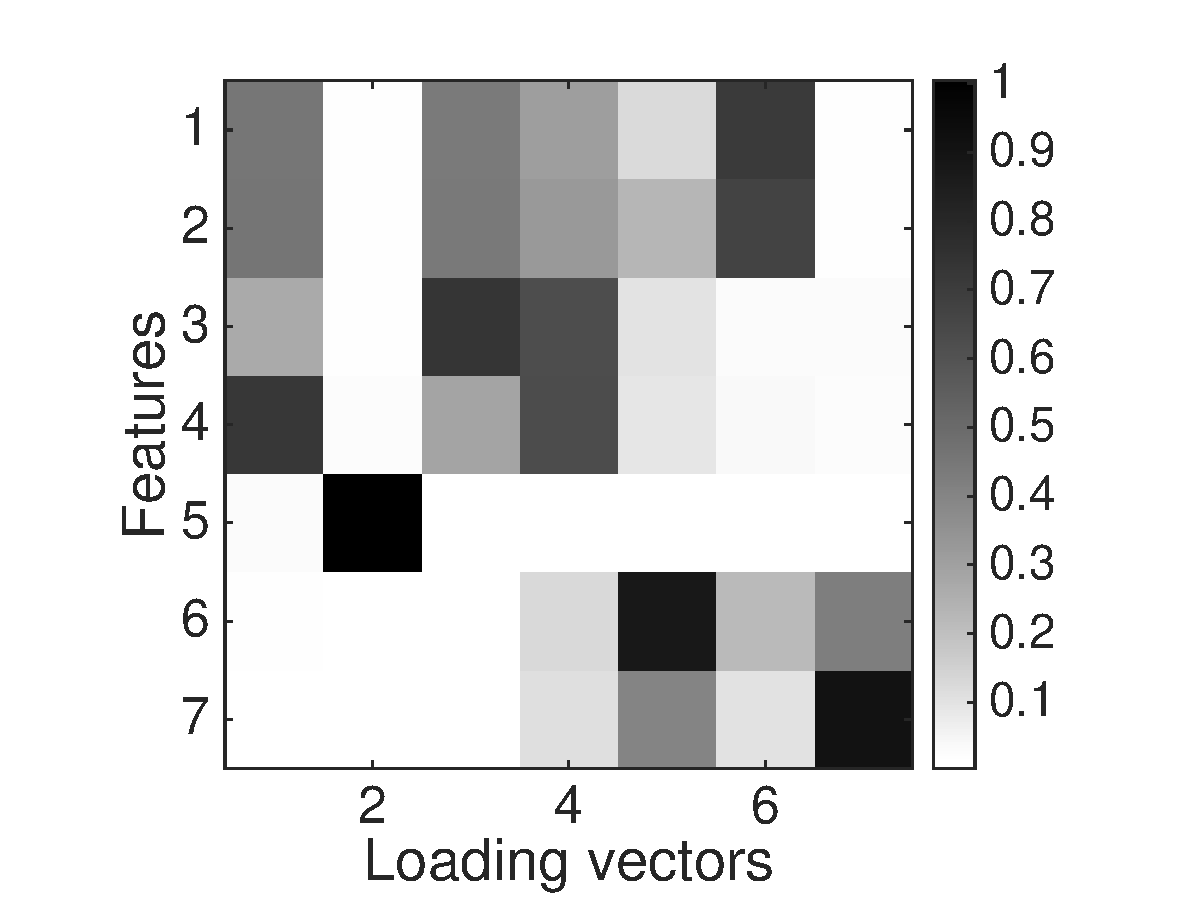
\includegraphics[height=50mm]{figure/new/Synthetic-Components-PCA}
\label{fig:pcs:PCA}
\caption{PCA}
\end{minipage}\hfill
\begin{minipage}{0.48\textwidth}
\centering
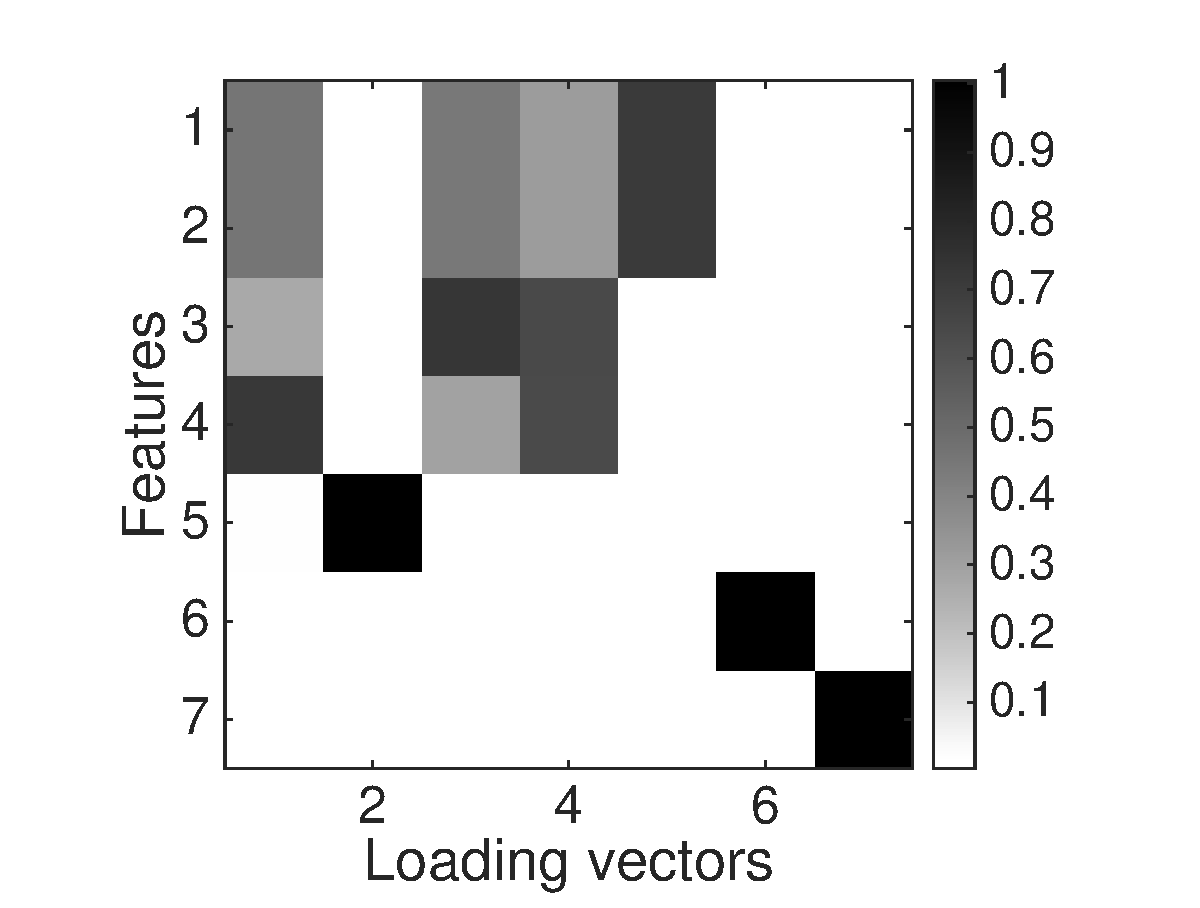
\includegraphics[height=50mm]{figure/new/Synthetic-Components-ASPCA-F}
\label{fig:pcs:ASPCA}
\caption{ASPCA}
\end{minipage}
\caption{Synthetic data and loading matrices obtained by PCA and ASPCA}
\label{fig:mappingmatrix}
\end{figure}

由\ref{equation:SPE}可知,SPE的计算并不需要通过计算两次空间投影后的向量,只需要计算一次空间变换后的长度即可。即SPE等于 ${\bf y}$ 在系数向量上的标量投影的平方和。因此我们可以认为,计算SPE的加和等式中,对于总和超过阈值有着突出贡献的加数对于该数据点被判别为异常点有很关键的作用。每个这样的加数,分别是数据点 ${\bf y}$ 在系数向量上投影的平方和,同时也是数据各个特征依据系数向量给予的组合方式之后所求出的值的平方。

因此,PCA判别异常除了数据无法被正常子空间所完全描述以外,还有另一种解释方法。即,数据点的各个特征按照一系列指定的参数关系相加之后所产生的一系列数值在正常情况下都是很小的,而在异常情况下,这一系列数值的平方和相加超过判定的阈值。也就是说,异常产生可以被视为是一些数据点违背了正常情况下数据所遵守的一些线性规律。

同样用之前关于行星轨迹的例子来解释,八大行星所遵循的是在与黄道平面垂直的$z$轴的值基本为零,而冥王星则常常打破这个约束。

但是在更普遍的场景下,所提到的这些PCA所挖掘的线性规律,也即异常主成分的系数向量,也即异常子空间的基向量是非常复杂的,涉及到很多原本的特征,远远不想行星轨迹那样只涉及到一个$z$轴上的运动值。因此,异常点仍然无法解释。为了使他们变得清晰简洁,我们希望他们能够具有稀疏的性质。

因此,我们提出了我们自己的改进模型。新的模型希望获取异常子空间的一组新的基向量,这些基向量同时具有正交稀疏的性质。这种基向量所构造的异常子空间将能够同时完成异常检测和异常诊断任务。正交性确保等式~\ref{equation:SPE}成立,而稀疏性提供保证了每一条线性关系的简明易读。我们将该模型称为异常子空间稀疏PCA即Abnormal Subspace Sparse PCA(ASPCA)。

对于一个异常而言,他对线性关系的违背超过了阈值,这里涉及到的线性关系可能只是少数几条,但也可能出现涉及很多的情况。我们判断是某条线性关系否涉及的依据是对该关系的违背情况与阈值的相对大小。理论上,可能会出现很多关系的违背影响力都很大的情况,也可能出现大量关系的违背情况都很微小,但相加的总和却超过了阈值的情况。但实际使用中发现,大多数异常都还是在部分特征上有所体现,因此较少出现以上所陈述的两种情况。而如何在模型中考虑这种问题,即在关于异常子空间基向量的稀疏性与正交性约束之外再加上一条,异常在基向量的投影的稀疏性,也在我们的后续工作中继续研究。 

我们构造了一个由500个正例与15个反例构成的数据集来进行演示。其中最前面的100歌正例如图~\ref{fig:synthesized_data})所示。每一个数据点有七个特征,分别命名为$A$ 到 $G$,且正常的数据通过4种模式进行生成,即$A \approx B$,$D \approx C + A$,$F \approx 0$,$G \approx 0$。反例则有三种类型,分别通过打破前三种模式进行生成。通过PCA得到的主成分参数矩阵如图~\ref{fig:pcs:PCA}所示,其中PCA得到的靠后的四个主成分即异常主成分,很难进行解读。当我们通过我们之后将会介绍的算法,根据我们要求稀疏性和正交性的ASPCA模型所得到的主成分参数矩阵如图~\ref{fig:pcs:ASPCA}所示,这样得到的靠后的四个异常主成分的系数向量,将可以很好的在异常检测的同时完成异常诊断任务。

ASPCA模型将异常的解释分成两个步骤,首先,我们分析样本在哪些异常基向量上的投影,即对线性关系的违背,对于SPE有很高的贡献,这依据的是等式~\ref{equation:SPE}。然后,阐释这些不同的线性关系。

\begin{figure}
	\centering
	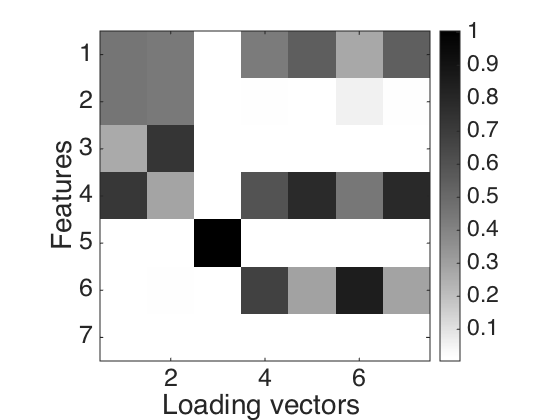
\includegraphics[height=30mm]{figure/new/Synthetic-Components-JSPCA}
\caption{Loading matrix obtained by JSPCA}
\label{fig:loading matrix:synthetic}
\end{figure}

相关工作中所提到的 Jiang 等人所做的工作\cite{jiang2013family},即联合稀疏PCA(JSPCA)同样是通过获取异常子空间的稀疏表达来进行异常分析。但他们的主要思路是从整体上用较少的特征来近似表达异常子空间,这种方式下,所有的系数向量都是由相同的少数几个特征来进行表达如图\ref{fig:loading matrix:synthetic}。尽管JSPCA获取到了与异常相关联的特征维度,但是他有两个主要限制。其一,JSPCA所识别的特征是从数据集中所有异常角度进行考虑的,即他所捕捉的是所有异常所体现的主要特征。当异常存在不同类别时,不同种类的异常应当有不同的表现,这在网络入侵检测,系统异常检测等场景下也是很普遍的现象。而对于这样的情况,JSPCA无法给不同种类的异常不同的解释。对于一个无监督异常检测任务,JSPCA显然不能假定异常只有一种类别内。其二,JSPCA识别了异常的主要相关特征,但并没有阐释这样的特征是如何导致记录点被判定为异常,即没有给出直接的依据。

\subsection{ASPCA模型}

以上,我们提出了一个新的异常检测解释模型ASPCA,以下我们将介绍ASPCA的两种求解方式。

首先,对于正常空间稀疏PCA问题的求解,普遍有两种思路,其一是整体解法,其二是逐步解法\cite{SPCA-SDP}。

整体解法的思路是构造一组子空间的稀疏基向量,在这组基向量上,数据将能够最好的进行还原,即原始数据与投影后的数据偏差最小。如果按照这样的思路进行计算,ASPCA模型需要的是投影后本身最小的一个子空间,因为异常子空间本身就是原始数据与正常子空间投影的偏差。但是,这种解法并没有约束子空间的各个基向量具有正交性质,而在添加了正交约束后,原本的优化方法不再适用。因此我们选择了另一种思路,即逐步解法。

逐步解法的思路是每次只计算求解一个稀疏基向量,该基向量具有稀疏的性质,并且数据在该基向量上有最大的方差。随后将已经被求解出的基向量所覆盖的变化从数据中剔除出去,再用修改后的数据求出第二个基向量,同样的步骤继续下去直到所有基向量都被求解出来。如果按照这样的思路,ASPCA模型同样需要考虑基向量正交的问题,而一般所用的修改数据的方式来逐个求解基向量的方式无法保证该约束,因此我们不采用修改数据的方式,而是直接添加正交性要求,即:当前求解出的基向量必须与之前已经求解的基向量正交。并且,我们可以通过一些条件的放松,利用半正定规划求解该优化问题。

总之,我们通过在逐步解法添加正交性约束,去除掉修改数据的步骤,实现了我们ASPCA模型的第一个解法,我们将其称之为${\bf 前向ASPCA}$ 即 ASPCA-F。

给定数据的协方差矩阵 ${\bf A}$ ,以及对稀疏性的要求参数 $k$,对于每一个基向量${{\bf v}_i},i = 1,...,p$的计算,ASPCA-F所要优化的目标函数为:

\begin{equation}
\label{equation:typical_MSPCA-F}
\begin{split}
& \argmax_{{\bf v}_i}\ {\bf v}_i^T{\bf A}{\bf v}_i\\
 s.t. & \ {\bf v}_i^T{\bf v}_i=1,\ Card({\bf v}_i)\leq k, \\
 &\ {\bf v}_i^T{\bf v}_j=0\ \forall 1\leq j<i. 
 \end{split}
\end{equation}

ASPCA-F所获取的$p$条向量中,靠前先获取的向量构成正常子空间,而靠后的向量构成异常子空间。

ASPCA-F的主要问题在于,它优先获取了正常子空间的稀疏表示,但这并不是我们所需要的。而如果对于ASPCA-F先求解出来的向量不给予稀疏性的限制,而只对后获取的用来构建异常子空间的向量加上稀疏性限制,由于异常子空间需要与正常子空间正交,因此会受到正常子空间影响。总之,求解异常子空间之前需要先求解正常子空间是导致ASPCA-F不令人满意的主要原因。

因此,我们提出了另一种解法,即直接求解异常子空间,即先求解方差最小的主成分,将之前的整个求解过程逆转过来。我们将这种解法称为${\bf 后向ASPCA}$即$ASPCA-B$。这种求解方式下,优先保证异常子空间的稀疏性。由于PCA求解原本就可以从最小主成分开始计算,正如\ref{prop:reverse}所证,因此ASPCA-B从后往前计算也是合理的。其中PCA所求解的主成分所对应的向量就是数据协方差矩阵的特征向量,而构成正常子空间的基向量就是最大的若干个特征向量,异常子空间则是较小的特征向量。因此,我们证明的是对于协方差矩阵${\bf A}$,可以先求出最小的若干特征值所对应的特征向量,再求出较大的特征值与特征向量。

\begin{proposition}
\label{prop:reverse}
给定协方差矩阵 ${\bf A} = {\bf D}^T{\bf D}$,如果我们已经提取了对应于$n-k-1$个最小特征值的正交特征向量 ${\bf v}_{k+1},{\bf v}_{k+2},....,{\bf v}_n$,剩余的没有被提取的特征值从大到小为 $\lambda_1 \geq \lambda_2 \geq ... \geq \lambda_k$,对应的特征向量为 ${\bf v}_1, {\bf v}_2,....,{\bf v}_k$,所有特征向量相互垂直 ,则表达式\ref{equation:proposition:init} 的解即为特征值$\lambda_k$所对应的特征向量.
\begin{equation}
\begin{split}
 & \argmin_{{\bf v}}\ {\bf v}^T{\bf A}{\bf v}\\
 s.t. & {\bf v}^T{\bf v} =1,\ {\bf v}^T{\bf v}_i=0\ \forall k<i\leq n
\end{split}
\label{equation:proposition:init}
\end{equation}
\end{proposition}
\begin{proof}
将 ${\bf v}$ 投影到 $({\bf v}_1,...,{\bf v}_n)$,可以得到 ${\bf v} = \sum_{i=1}^{n} \alpha_i {\bf v}_i$,其中 $\alpha_i = {\bf v}^T{\bf v}_i$。又因为有限制条件 ${\bf v}^T{\bf v}_i=0\ \forall k<i\leq n$ 因此可得 $\alpha_i = 0\  \forall k<i\leq n$,即可得${\bf v} = \sum_{i=1}^{k} \alpha_i {\bf v}_i$。

优化目标${\bf v}^T{\bf A}{\bf v}$ 可以展开为:

\begin{equation*}
\begin{split}
 & {\bf v}^T{\bf A}{\bf v}\\
 =& (\sum_{i=1}^{k} \alpha_i {\bf v_i})(\sum_{i=1}^{k} \alpha_i {\bf A}{\bf v}_i)\\
 =& (\sum_{i=1}^{k} \alpha_i {\bf v}_i)(\sum_{i=1}^{k} \alpha_i \lambda_i  {\bf v}_i)\\
 =& \sum_{i=1}^{k} \alpha_i^2 \lambda_i {\bf v}_i^T {\bf v}_i + \sum_{i=1}^{k} \sum_{j=1,j \neq i}^{k} \alpha_i \alpha_j \lambda_j {\bf v}_i^T {\bf v}_j
\end{split}
\end{equation*}

由于${\bf v}_i^T{\bf v}_j=0, i \neq j$,因此可得 $\sum_{i=1}^{k} \sum_{j=1,j \neq i}^{k} \alpha_i \alpha_j \lambda_j {\bf v}_i^T {\bf v}_j = 0$。由此得到:

\begin{equation}
\label{equa:vAv}
{\bf v}^T{\bf A}{\bf v} = \sum_{i=1}^{k} \alpha_i^2 \lambda_i
\end{equation}

由于 $\lambda_i \geq \lambda_k \ \forall i\leq k$,因此可得:

\begin{equation*}
\begin{split}
	{\bf v}^T{\bf A}{\bf v} = \sum_{i=1}^{k} \alpha_i^2 \lambda_i \geq \sum_{i=1}^{k} \alpha_i^2 \lambda_k = \lambda_k  \sum_{i=1}^{k} \alpha_i^2
\end{split}
\end{equation*}

由于${\bf v}^T{\bf v} = \sum_{i=1}^{k} \alpha_i^2 = 1$,可以得到:

\begin{equation}
\label{equa:geq}
	{\bf v}^T{\bf A}{\bf v} \geq \lambda_k 
\end{equation}

由于${\bf v}_k$ 符合${\bf v}$所需要满足的约束,因此是优化问题的待选解之一,但将${\bf v}_k$代入后的值一定不会优于最优解。因此可得:

\begin{equation}
\label{equa:leq}
\min_{\bf v}{{\bf v}^T{\bf A}{\bf v}} \leq {\bf v}_k^T{\bf A}{\bf v}_k = \lambda_k
\end{equation}

结合两个方向的不等式,即表达式~\ref{equa:geq}与表达式~\ref{equa:leq}可以得到:

\begin{equation}
\label{equa:equalK}
\min_{\bf v}{{\bf v}^T{\bf A}{\bf v}} = \lambda_k
\end{equation}

假设最优值为 $\hat{{\bf v}} = \sum_{i=1}^{k} \hat{\alpha}_i {\bf v}_i$,由表达式~\ref{equa:vAv} 可知有$\hat{{\bf v}}^T{\bf A}\hat{{\bf v}} = \sum_{i=1}^{k} \hat{\alpha}_i^2 \lambda_i$ ,又通过表达式~\ref{equa:equalK} 可知有$\hat{{\bf v}}^T{\bf A}\hat{{\bf v}} = \lambda_k$,因此可得:
\begin{equation*}
\begin{split}
\lambda_k - \sum_{i=1}^{k} \hat{\alpha}_i^2 \lambda_i = \sum_{i=1}^{k} \hat{\alpha}_i^2 (\lambda_k - \lambda_i) = 0 
\end{split}
\end{equation*}
由于 $\lambda_k - \lambda_i\leq 0,\forall i<k$,所以 $\hat{\alpha}_i^2 (\lambda_k - \lambda_i) $ 每一项都大于等于零,而求和是零,因此每一项都为零。因此可得 $\hat{\alpha}_i \neq 0$ 的必要条件是 $\lambda_i = \lambda_k$。因此可知,$\hat{{\bf v}}$ 是特征值为 $\lambda_k$  所对应的特征向量的线性组合。因而 $\hat{{\bf v}}$ 自己也是一个特征向量,对应的特征值为$\lambda_k$。
\end{proof}

显然,我们的证明对于 $k=n$ 也是成立的。 通过表达式~\ref{equation:proposition:init},我们可以从小到大的逐个计算特征值所对应的特征向量。在表达式~\ref{equation:proposition:init} 的基础上加上稀疏性限制则形成了ASPCA-B的优化目标。

给定协方差矩阵 ${\bf A}$ 以及稀疏性限制参数 $k$, 对于每一个基向量 ${\bf v_i},\ i = 1,...,d$ 的计算, ASPCA-B的优化目标函数为:
\begin{equation}
\label{equation:typical_MSPCA-B}
\begin{split}
 &\argmin_{{\bf v}_i}\ {\bf v}_i^T{\bf A}{\bf v}_i\\
s.t. &\ {\bf v}_i^T{\bf v}_i=1,  Card({\bf v}_i)\leq k. \\
& {\bf v}_i^T{\bf v}_j=0\ \forall 1\leq j<i,
 \end{split}
\end{equation}

ASPCA-B所提取的前 $d$ 个向量 $\bf{v}_1...\bf{v}_d$ 构成了我们所需要的异常子空间 ${\bf S}_a$,而剩余的补空间则是正常子空间。我们直接使用数据点在异常子空间下的投影来完成异常的检测与解释。

\chapter{ASPCA模型}

之前所提出了ASPCA-F与ASPCA-B本身并不能很好的被优化,需要对条件进行一些放松。我们所做的放松处理是参考自SPCA算法的处理\cite{SPCA-SDP}。而在求得ASPCA-F与ASPCA-G的解后,我们还尝试了从整体角度再对之前逐步求解的结果进行一次优化。最后的这一步优化是通过保证新得到的基向量所张成的空间与之前所求解的异常子空间一致,以稀疏性为目标的一个优化,计算过程受到 \cite{SPCA-2006}启发,通过交替最小化求解。

\section{求解ASPCA-F}

我们首先将表达式~\ref{equation:typical_MSPCA-F} 中的优化目标转化为一个SDP形式的优化目标。

当求解第$i$个基向量时,之前已经求出的基向量组成一个矩阵 ${\bf V}_{i-1} = ({\bf v}_1, {\bf v}_2, ... ,{\bf v}_{i-1})$,则正交约束条件可以表示为 ${\bf V}_{i-1}^T{\bf v}_i={\bf 0}$ 也即 $||{\bf V}_{i-1}^T{\bf v}_i||_2=0$。

定义 ${\bf v}_i{\bf v}_i^T={\bf X}$,定义${\bf R}_{i-1} = {\bf V}_{i-1}{\bf V}_{i-1}^T$。可以将原本的优化目标与约束转化成用${\bf X}_i$来表示。例如优化目标可以转化为:

\begin{equation*}
\begin{split}
{\bf v}_i^T{\bf A}{\bf v}_i & = Tr({\bf v}_i^T{\bf A}{\bf v}_i)\\
& = Tr({\bf A}{\bf v}_i{\bf v}_i^T)\\
& =Tr({\bf A}{\bf X}_i)
\end{split}
\end{equation*}

该转换合法的原因是计算矩阵的迹时,矩阵满足交换律,即$Tr(\bf{AB})=Tr(\bf{BA})$。因为矩阵的迹是$A$与$B^T$中同行同列元素相乘求和的结果,交换后$A^T$与$B$同行同列的元素任然相同,求和结果不变。

各个限制条件可以转化为:
\begin{equation*}
	\begin{split}
		{\bf v}_i^T{\bf v}_i &=Tr({\bf v}_i^T{\bf v}_i)=Tr({\bf v}_i{\bf v}_i^T) = Tr({\bf X}_i)=1\\
		Card({\bf v}_i{\bf v}_i^T) &= Card({\bf X}_i) \leq k^2 \\
		||{\bf V}_{i-1}^T{\bf v}_i||_2 &=({\bf V}_{i-1}^T{\bf v}_i)^T({\bf V}_{i-1}^T{\bf v}_i) \\
		&=Tr(({\bf V}_{i-1}^T{\bf v}_i)^T({\bf V}_{i-1}^T{\bf v}_i))\\
		& =Tr({\bf V}_{i-1}{\bf V}_{i-1}^T{\bf v}_i{\bf v}_i^T)\\
		& =Tr({\bf R}_{i-1}{\bf X}_i)=0
	\end{split}
\end{equation*}

其中第二项限制条件,与原本的约束条件是等价的,因为${\bf X}_i$上任意一项是${\bf v}_i$中所取的两个值的积,因此如果乘积为零,则必然是因为其中一个乘数为零,因此当少于有$k^2$个非零项时,乘数中有少于$k$个非零项,反之亦然。

在以上约束下所求出的优化问题$\argmax_{{\bf X}_i \in \mathbb{S}^p}\ Tr({\bf A}{\bf X}_i)$的最优解${\bf {\hat X}}_i$ 还需要约束其为半正定矩阵,并且有$rank({\bf X})=1$,这样才能从转换后问题的最优解${\bf {\hat X}}$通过特征值分解得到表达式\ref{equation:typical_MSPCA-F}的最优解${\bf v}_i$。

因此,原本的ASPCA-F优化问题从表达式\ref{equation:typical_MSPCA-F}可以等价转换到表达式\ref{equation:aspca_sdp}。


\begin{equation}
\label{equation:aspca_sdp}
\begin{split}
 & \argmax_{{\bf X}_i \in \mathbb{S}^p}\ Tr({\bf A}{\bf X}_i)\\
 & s.t.\ {\bf X}_i\succeq0, rank({\bf X}_i)=1, \ Tr({\bf X}_i)=1, Card({\bf X}_i) < k^2\\
\end{split}
\end{equation}

之后的转换是对原表达式条件的一些放松,不再是等价转换,我们所做的放松参照的是SPCA\cite{SPCA-SDP}中相应的处理。首先我们将稀疏性条件放松为$||{\bf X}_i||_{1,1}<k$,再将其从约束条件转移到优化目标中,通过参数$\lambda$与原本的优化目标结合。当$\lambda$越大时,结果的稀疏性更好,当其更接近零时,结果与PCA的结果更接近。另外,为了问题能够在凸规划下可解,我们直接去掉了约束条件$rank({\bf X}_i)=1$。这样就形成了最终真正求解的表达式~\ref{equation:aspca_f_sdp_final}。我们可以通过半正定规划,即SDP(Semidefinite Programming)求解该优化问题。

\begin{equation}
\label{equation:aspca_f_sdp_final}
\begin{split}
& \argmax_{{\bf X}_i \in \mathbb{S}^p}\ Tr({\bf A}{\bf X}_i)-\lambda ||{\bf X}_i||_{1,1}\\
& s.t.\ {\bf X}_i\succeq0,\ Tr({\bf X}_i)=1, Tr({\bf R}_{i-1}{\bf X}_i)=0\\
\end{split}
\end{equation}

之前提到,我们将${\bf X}_i$关于矩阵秩的约束去掉了。首先,如果没有稀疏性的目标,即普通的PCA问题求解,该条件是可以被去掉的,所求出的最优解矩阵${\bf \hat{X}}_i$可以通过特征值分解,分解为协方差矩阵${\bf A}$的第$i$个特征值的若干个互相垂直的特征向量所组成的矩阵。即还是求出了原本数据的主成分相对应的向量。而对于加入了稀疏约束后的问题,则可以选择对${\bf \hat{X}_i}$特征值分解得到的矩阵中最大特征值的特征向量作为这一步的解。

\section{求解ASPCA-B}

与求解ASPCA-F的优化目标,即表达式~\ref{equation:typical_MSPCA-F}类似, 我们将表达式~\ref{equation:typical_MSPCA-B}转化并最终放松到表达式~~\ref{equation:aspca_b_sdp_final}, 该优化目标同样可以通过SDP进行求解。
\begin{equation}
\label{equation:aspca_b_sdp_final}
\begin{split}
& \argmin_{{\bf X}_i \in \mathbb{S}^p}\ Tr({\bf A}{\bf X}_i)+\lambda ||{\bf X}_i||_{1,1}\\
& s.t.\ {\bf X}_i\succeq0,\ Tr({\bf X}_i)=1, Tr({\bf R}_{i-1}{\bf X}_i)=0\\
\end{split}
\end{equation}

\section{全局稀疏化优化}
定义 ${\bf V}=({\bf v}_1,...,{\bf v}_d)$ 为我们通过ASPCA-F或者ASPCA-B所获取的构成异常空间的基向量。而对于该异常空间而言,可以有不同的基来描述。定义一组异常空间的新正交基${{\bf c}_1,...,{\bf c}_d}$。有:

\begin{equation}
SPE= \sum_{i=1}^{d}({\bf v}_i^T {\bf y})^2 = \sum_{i=1}^{d}({\bf c}_i^T {\bf y})^2
\end{equation}

因此我们可以在逐步求解得到异常空间后,再对异常空间全局进行优化,寻找到稀疏性更好的一组正交基,而这组正交基同样可以用来表示SPE,即也能够进行异常的检测与解释。而为了得到这组新的正交基,我们需要对原来求得的基向量组进行正交变换,变换矩阵为正交矩阵${\bf X}$,则优化目标为:

\begin{equation}
\begin{split}
&\argmin_{{\bf X}}\ ||{\bf V}{\bf X}||_{1,1}\\
& s.t.\ {\bf X}^T{\bf X}=I
\end{split}
\end{equation}

定义我们所要获得的新基向量组${\bf C}={\bf V}{\bf X}$, 我们将问题转化为一个回归问题,即:

\begin{equation}
\begin{split}
&\argmin_{{\bf X},{\bf C}}\ ||{\bf V}-{\bf C}{\bf X}^T||_F+\mu||{\bf C}||_{1,1}\\
&s.t.\ {\bf X}^T{\bf X}={\bf I}
\end{split}
\label{equation:step2}
\end{equation}


表达式~\ref{equation:step2}所示的回归优化问题可以通过交替最小化法进行求解\cite{SPCA-2006}。初始时,我们设定 ${\bf X}$ 为单位矩阵, 设定 $\mu = ||{\bf V}||_F/||{\bf V}{\bf X}||_{1,1}$。在随后的迭代当中,我们逐渐减小$\mu$,从而确保最终所获得的${\bf C}$与之前所获得的基向量组${\bf V}$所表示的空间是相同的。

通过在ASPCA-F和ASPCA-B之后增加全局优化的步骤,我们收获了两种新的算法ASPCA-FG与ASPCA-BG。算法 1 和算法 2 详细描述了整个优化过程,其中${\bf A}$是输入数据矩阵的协方差矩阵,$d$ 是所需要获取的异常子空间的维度,$max\_iter$ 是全局优化步骤中交替迭代的次数。算法最终输出的矩阵${\bf V}$ 是构成异常子空间的基向量,同时也是相应的主成分的系数向量,同时也是异常所会违背的线性关系,通过这些向量,我们可以完成异常的检测与解释。

\renewcommand{\algorithmicrequire}{\textbf{Input:}}
\renewcommand{\algorithmicensure}{\textbf{Output:}}
\begin{algorithm}
\begin{algorithmic}[1]
    \caption{Forward Abnormal Subspace Sparse PCA with Global Optimization (ASPCA-FG)}
    \REQUIRE  ${\bf A},\ d,\ \lambda$, and $max\_iter$
    \ENSURE ${\bf V}$
    \FOR{$i=1$ to $p$}
	\STATE ${\bf V}_{i-1} \gets ({\bf v}_1,{\bf v}_2...{\bf v}_{i-1})$;
 	\STATE ${\bf R}_{i-1} \gets {\bf V}_{i-1}{\bf V}_{i-1}^T$;
	\STATE Optimize ${\bf v}_i$ with given ${\bf A},\ {\bf R}_{i-1}$ according to Eqn.~\ref{equation:aspca_f_sdp_final} using SDP;
    \ENDFOR
    \STATE ${\bf V} \gets ({\bf v}_{p-d+1},...{\bf v}_p)$;
    \STATE Optimize ${\bf X},\ {\bf C}$ with given ${\bf V},\ max\_iter$ according to Eqn.~\ref{equation:step2} using the alternating minimization scheme;
    \STATE ${\bf V} \gets {\bf C}{\bf X}$;
    \RETURN ${\bf V}$;
\end{algorithmic}
\end{algorithm}

\renewcommand{\algorithmicrequire}{\textbf{Input:}}
\renewcommand{\algorithmicensure}{\textbf{Output:}}
\begin{algorithm}
\begin{algorithmic}[1]
    \caption{Backward Abnormal Subspace Sparse PCA with Global Optimization (ASPCA-BG)}
    \REQUIRE  ${\bf A},\ d,\ \lambda$, and $max\_iter$
    \ENSURE ${\bf V}$
    \FOR{$i=1$ to $d$}
	\STATE ${\bf V}_{i-1} \gets ({\bf v}_1,{\bf v}_2...{\bf v}_{i-1})$;
 	\STATE ${\bf R}_{i-1} \gets {\bf V}_{i-1}{\bf V}_{i-1}^T$;
	\STATE Optimize ${\bf v}_i$ with given ${\bf A},\ {\bf R}_{i-1}$ according to Eqn.~\ref{equation:aspca_b_sdp_final} using SDP;
    \ENDFOR
    \STATE ${\bf V} \gets ({\bf v}_1,{\bf v}_2...{\bf v}_d)$;
    \STATE Optimize ${\bf X},\ {\bf C}$ with given ${\bf V},\ max\_iter$ according to Eqn.~\ref{equation:step2} using the alternating minimization scheme;
    \STATE ${\bf V} \gets {\bf C}{\bf X}$;
    \RETURN ${\bf V}$;
\end{algorithmic}
\end{algorithm}


\chapter{实验}

\subsection{数据集}
为了验证我们所提出的ASPCA模型,我们采用了一个人工数据集(在第二章中进行了介绍)以及两个真实数据集。真实数据集分别是一个医学数据集(恶性乳腺癌肿瘤细胞判定)以及一个网络入侵数据集(KDD99比赛数据集)。

乳腺癌判定数据集 {\bf Breast Cancer Wisconsin (Diagnostic) Data Set}  \cite{breast-cancer-data} 提供了很多特征来判定一个细胞群落是良性乳腺肿瘤细胞还是恶性乳腺肿瘤细胞。群落的特征主要是各个细胞外貌特征的一些统计值,例如细胞半径的平均值。一共有$3\times10$个特征,由是个个体特征以及三种统计值类型组合而成。特征包括:半径,质地,周长,面积,光滑度,紧密度,凹度,凹点,对称性以及分形维度。统计值类型包括均值,标准差,以及最值。一个异常检测任务的数据集需要有占主流的正常样本以及少量异常样本。因此,我们抽取了全部的357个良性样本以及前10个恶性样本。这种样本抽取方法与其他研究者\cite{Kriegel:2009:LLO, Amer:2013:EOS}相同。所有的30个实数特征值都进行的均值归零,并且将其进行缩放以保证其数值大小在$[-1, 1]$范围内。

{\bf KDD 99 入侵检测比赛数据集} \cite{cup1999data}  是一个在异常检测与入侵检测研究领域广泛使用的一个数据集。每一个样例都是一个访问连接,每一个这样的连接都被归入到正常类别或者是22种不同的攻击当中。22中不同的攻击又被归为4个大类当中,分别是阻断服务攻击(DoS),R2L攻击,U2R权限获取攻击,以及漏洞探测。我们选用了官方所提供的10\%数据集中全部的正常访问记录以及部分异常访问记录,没有选择全部的异常访问记录同样是为了构建一个由正常样例主导的异常检测数据集。我们选择了记录较多的一些攻击类型的前五百个攻击记录,攻击类型包括:\emph{smurf} ,\emph{neptune}, \emph{back}, \emph{teardrop}, \emph{satan}, \emph{ipsweep}, 以及 \emph{portsweep}。具体情况参见表格 \ref{Table:KDD 99}。

我们对于\emph{KDD}数据的预处理方式参考的是 \cite{jiang2013family}中的做法。该数据集总共有41个特征,其中包括7个类型特征,我们将这些类型特征转变为数值化的特征。例如,对于连接类型特征,TCP用数值0代替,UDP用1代替,ICMP用2代替。也可以有有别的处理方法,例如对于连接类型特征,将其转变为三个不同的数值特征,分别赋予1或0代表不同的类型归属。但在该工作当中,我们还是按照我们对比方法的处理方案。但在我们之后的异常解释当中可以看出,这一类特征在进行这样的数值化处理后,没有能够在异常检测中发挥作用。除此之外,我们还对一些数值偏向指数分布的特征进行了对数化处理,包括\emph{duration}(连接时长),  \emph{src\_bytes}(连接发送字节数),  \emph{dst\_bytes}(连接返回字节数)。另外,所有特征都进行了均值归零处理,并且进行了缩放以保证其数值大小在$[-1, 1]$范围内。

\begin{table}
\small
\centering
\caption{Statistics of KDD99 and the relevant features identified by JSPCA}
\label{Table:KDD 99}
\begin{tabular}{|c|c|c|c|}
\hline
Categories & \begin{tabular}[c]{@{}c@{}}\# \\Records \end{tabular}  & Types                                                                                                                                                             & \begin{tabular}[c]{@{}c@{}}Relevant Features \\ (JSPCA)\end{tabular}                                                                           \\ \hline
Normal     & 97,277 &                                                                                                                                                                   &                                                                                                                                                \\ \hline
DoS        & 2,264  & \begin{tabular}[c]{@{}c@{}}smurf(500),\\neptune(500),\\ back(500),\\ teardrop(500),\\ pod(264)\end{tabular}                                                      & \begin{tabular}[c]{@{}c@{}}\emph{service}, \\ \emph{src\_bytes},\\ \emph{dst\_bytes},\\ \emph{count}, \emph{srv\_count},\\ \emph{dst\_host\_count},\\ \emph{dst\_host\_srv\_count}\end{tabular} \\ \hline
Probe      & 1,731  & \begin{tabular}[c]{@{}c@{}}satan(500),\\ ipsweep(500),\\ portsweep(500),\\ nmap(231)\end{tabular}                                                                 & \emph{source\_bytes}                                                                                                                                  \\ \hline
U2R        & 52     & \begin{tabular}[c]{@{}c@{}}buffer\_overflow(30),\\ loadmodule(9),\\ perl(3), rootkit(10)\end{tabular}                                                             & \begin{tabular}[c]{@{}c@{}}\emph{duration},\\ \emph{src\_bytes},\\ \emph{dst\_bytes},\\ \emph{dst\_host\_count},\\ \emph{dst\_host\_srv\_count}\end{tabular}                      \\ \hline
R2L        & 1,126  & \begin{tabular}[c]{@{}c@{}}ftp\_write(8),\\ guess\_passwd(53),\\ imap(12), \\ multihop(7),\\ phf(4), spy(2),\\ warezclient(1,020),\\ warezserver(20)\end{tabular} & \begin{tabular}[c]{@{}c@{}}\emph{duration}, \emph{service},\\ \emph{src\_bytes},\\ \emph{dst\_bytes},\\ \emph{dst\_host\_count},\\ \emph{dst\_host\_srv\_count}\end{tabular}             \\ \hline
\end{tabular}
\end{table}

\subsection{对比方法}

We compared our proposed ASPCA models with the standard PCA model for detection and sparsity performance,  and with two state-of-the-art analytical models on PCA results: the JSPCA model \cite{jiang2013family} and a decision tree model used in \cite{XuWei-SOSP} for interpretation performance. For the decision tree model, we formed the training set with all predicted normal records and anomalies returned by our ASPCA model as negative and positive samples, respectively. Then the decision trees were trained using the CART model from MATLAB and trimmed manually for the best interpretation.

The parameters used in our model were listed in Table~\ref{table:parameters} and discussed in Section~\ref{sec:parameter}. The number of PCs used in PCA equals the total number of features minus the number of abnormal PCs for all datasets. The results of JSPCA on the synthetic data were obtained by choosing the best performed parameters, and we directly reported their results on KDD99 in \cite{jiang2013family}.   Note that, our ASPCA models make no assumptions on the anomalies in the dataset, and we built one model on the entire KDD99 dataset with anomalies from all different categories, whereas JSPCA built four models on KDD99, each including anomalies for a single major attacking category \cite{jiang2013family}.

\begin{table}
\small
\centering
\caption{Parameters}
\begin{tabular}{|c|c|c|}
\hline
              & \# abnormal PCs & $\lambda$ \\ \hline
Synthetic     & 4               & 5         \\ \hline
Breast-Cancer & 10              & 5         \\ \hline
KDD99        & 35              & 100       \\ \hline
\end{tabular}
    \label{table:parameters}
\end{table}

Finally, we implemented all methods with MATLAB and CVX, and performed all experiments on a laptop computer with 16 GB memory and a Intel(R) Core(TM) i7-4870HQ 2.50GHz CPU.

\subsection{实验结果}

\subsubsection{异常检测}
We first compared the various ASPCA models with the standard PCA model on the anomaly detection performance. Because all models can obtain a perfect ROC
curve for the Synthetic data, we only show the ROC curves on Breast-Cancer and KDD99 in Figure~\ref{fig:cancer:roc} and Figure~\ref{fig:kdd99:roc}, respectively. Note that,
since ASPCA-F and ASPCA-FG use the same abnormal subspace to detect anomalies, their ROC curves are identical which are labeled as ASPCA-F(G). Similarly, the ROC curves of ASPCA-B and ASPCA-BG are labeled as ASPCA-B(G). From Figure~\ref{fig:cancer:roc}, we can see that our proposed ASPCA-F(G) and ASPCA-B(G) models performed similarly or even better than PCA on anomaly detection for both datasets.

\begin{figure}
\centering
  \subcaptionbox{Breast-Cancer\label{fig:cancer:roc}}[3cm] 
  {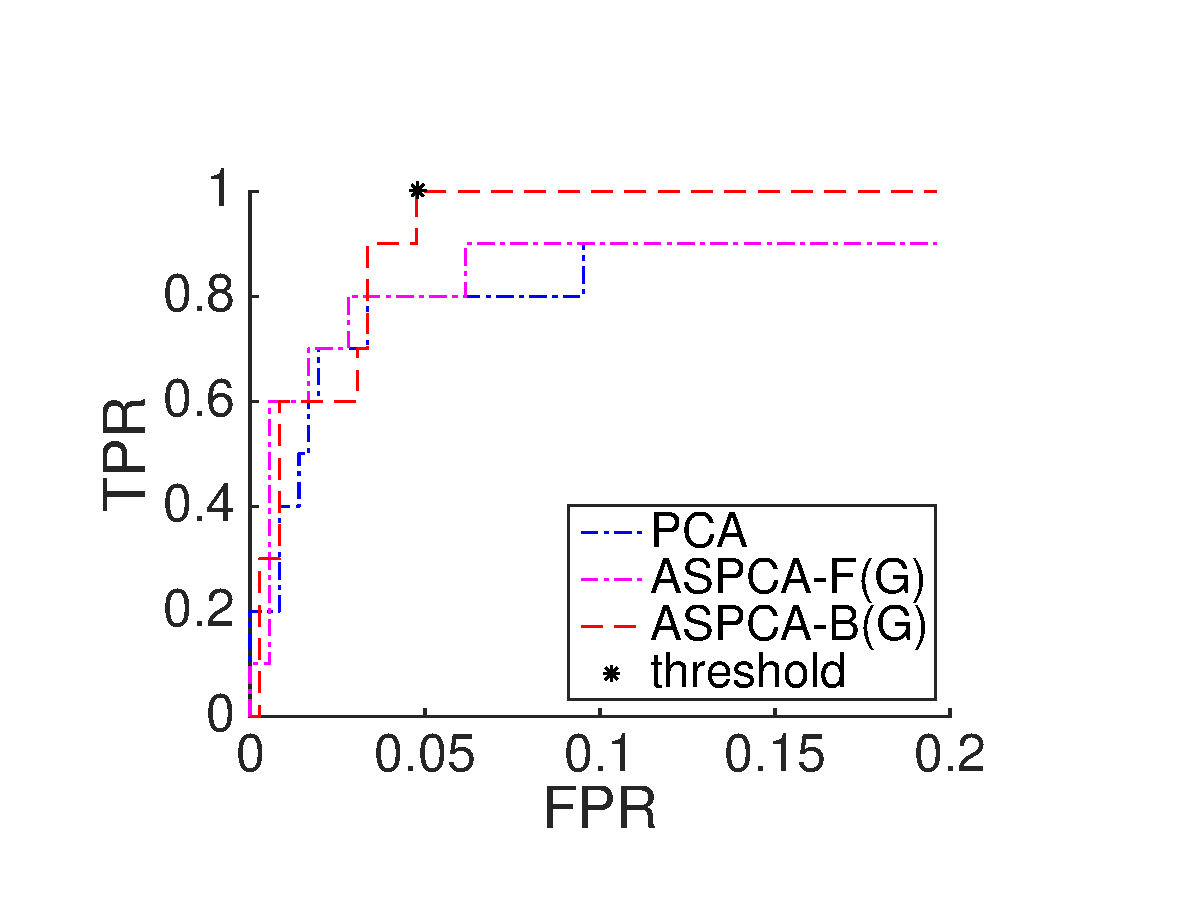
\includegraphics[width=40mm]{figure/new/Cancer-AUC-5}}
    \subcaptionbox{KDD99\label{fig:kdd99:roc}}[3cm] 
  {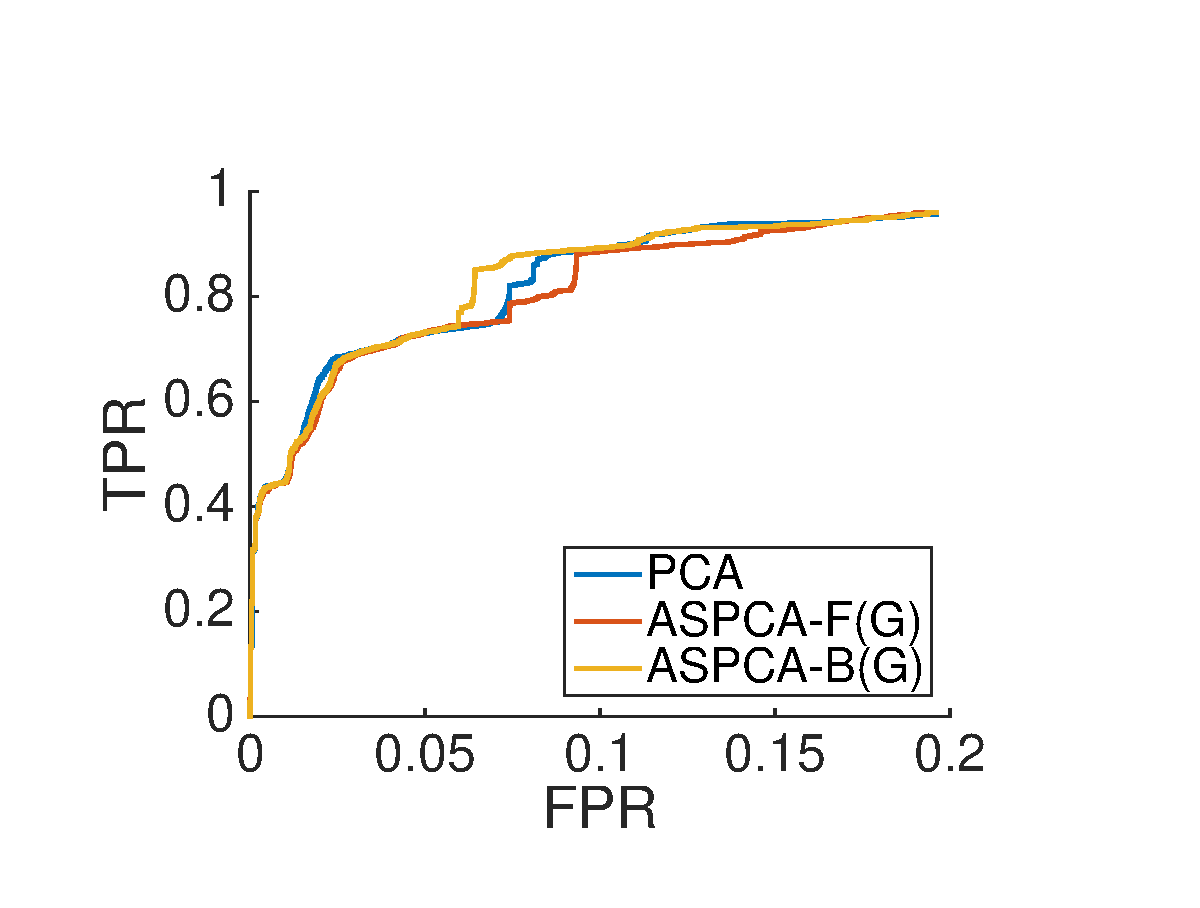
\includegraphics[width=40mm]{figure/new/KDD-AUC-100}}
\caption{ROC curves}
\label{fig:detection performane}
\end{figure}

\subsubsection{稀疏性}
The next set of experiments were designed to compare the sparsity of the loading matrix generated by various ASPCA models and we used the result of PCA as our baseline.  We used three metrics to evaluate the sparsity of the loading matrix of the abnormal PCs, namely,  $||V||_{1,1}$, $Card_{0.1}$ (number of entries with absolute values bigger than 0.1), and $Card_{0.01}$ (number of entries with absolute values bigger than 0.01), and showed the results in Table~\ref{table:sparsity}. We can see that all ASPCA models improved the sparsity of the loading matrix greatly over the baseline. For all datasets, the ASPCA-B model achieved better sparsity performance than the ASPCA-F model. The global optimization step improved $||V||_{1,1}$ values for both models on Breast-Cancer and KDD99. However, in terms of cardinality, ASPCA-FG performed worse than ASPCA-F on Breast-Cancer. The global optimization step achieved the largest sparsity improvement on KDD99, as it has more abnormal PCs than the other two datasets leaving more room for the global optimization. Overall, the ASPCA-BG model achieved the best sparsity performance.

The loading matrices returned by PCA and ASPCA-B (the other three ASPCA models have very similar results) on the Synthetic data are shown in Figure~\ref{fig:mappingmatrix}, and the loading matrices returned by PCA, ASPCA-F, ASPCA-B, ASPCA-FG, ASPCA-BG on Breast-Cancer and KDD99 are shown in Figure~\ref{fig:components}. We can see that ASPCA-F usually leaves some loading vectors with poor sparsity towards the end, which should be avoided as they are part of abnormal subspace. On the contrary, ASPCA-B leaves the loading vectors not so sparse towards the beginning, which need no interpretation as they belong to the normal subspace.

\begin{table}
\small
\caption{Sparsity on Synthetic data, Breast-Cancer, and KDD99}
\begin{tabular}{|l|l|l|l|l|}
\hline
dataset                        & method   & $||V||_{1,1}$ & $card_{0.1}$ & $card_{0.01}$ \\ \hline
\multirow{5}{*}{Synthetic}     & PCA      & 7.07    & 16        & 24           \\ \cline{2-5}
		                       & ASPCA-F  & 5.54    & 9           & 9           \\ \cline{2-5}
		                       & ASPCA-B  & 5.31    & 8          & 8           \\ \cline{2-5}
		                       & ASPCA-FG & 5.54    & 9           & 9           \\ \cline{2-5}
		                       & ASPCA-BG & 5.31    & 8           & 8           \\ \hline
\multirow{5}{*}{Breast-Cancer} & PCA      & 34.22    & 111        & 237           \\ \cline{2-5}
		                       & ASPCA-F  & 17.23    & 33           & 50           \\ \cline{2-5}
		                       & ASPCA-B  & 12.31    & 18          & 18           \\ \cline{2-5}
		                       & ASPCA-FG & 16.50    & 36           & 63           \\ \cline{2-5}
		                       & ASPCA-BG & 12.31    & 18           & 18           \\ \hline
\multirow{5}{*}{KDD99}        & PCA      & 97.33    & 248          & 691           \\ \cline{2-5}
                               & ASPCA-F  & 55.01    & 96           & 265           \\ \cline{2-5}
                               & ASPCA-B  & 54.52    & 101          & 215           \\ \cline{2-5}
                               & ASPCA-FG & 42.77    & 58           & 159           \\ \cline{2-5}
                               & ASPCA-BG & 43.05    & 57           & 157           \\ \hline
\end{tabular}
\label{table:sparsity}
\end{table}

\begin{figure*}
	\centering
    \subcaptionbox{}{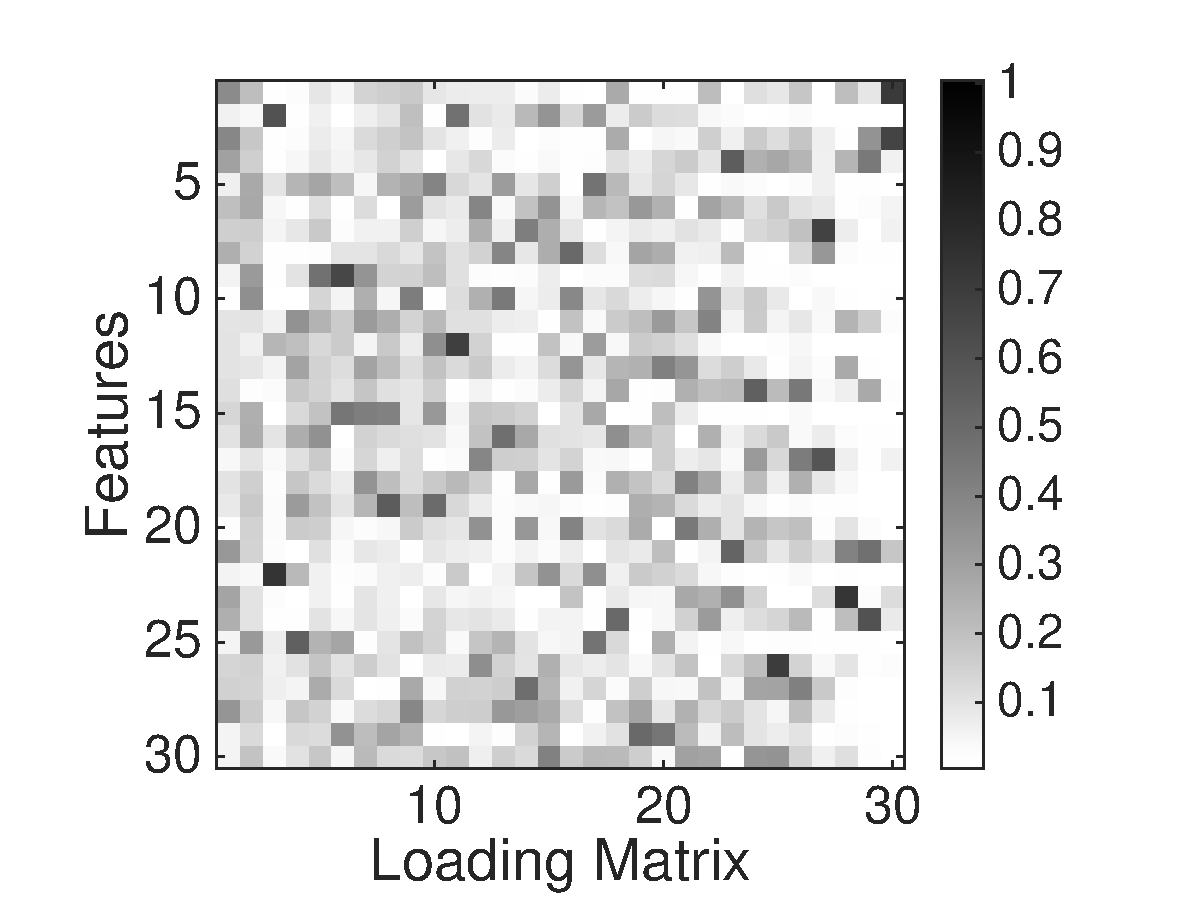
\includegraphics[width=35mm]{figure/new/Cancer-Components-PCA}}
    \subcaptionbox{}{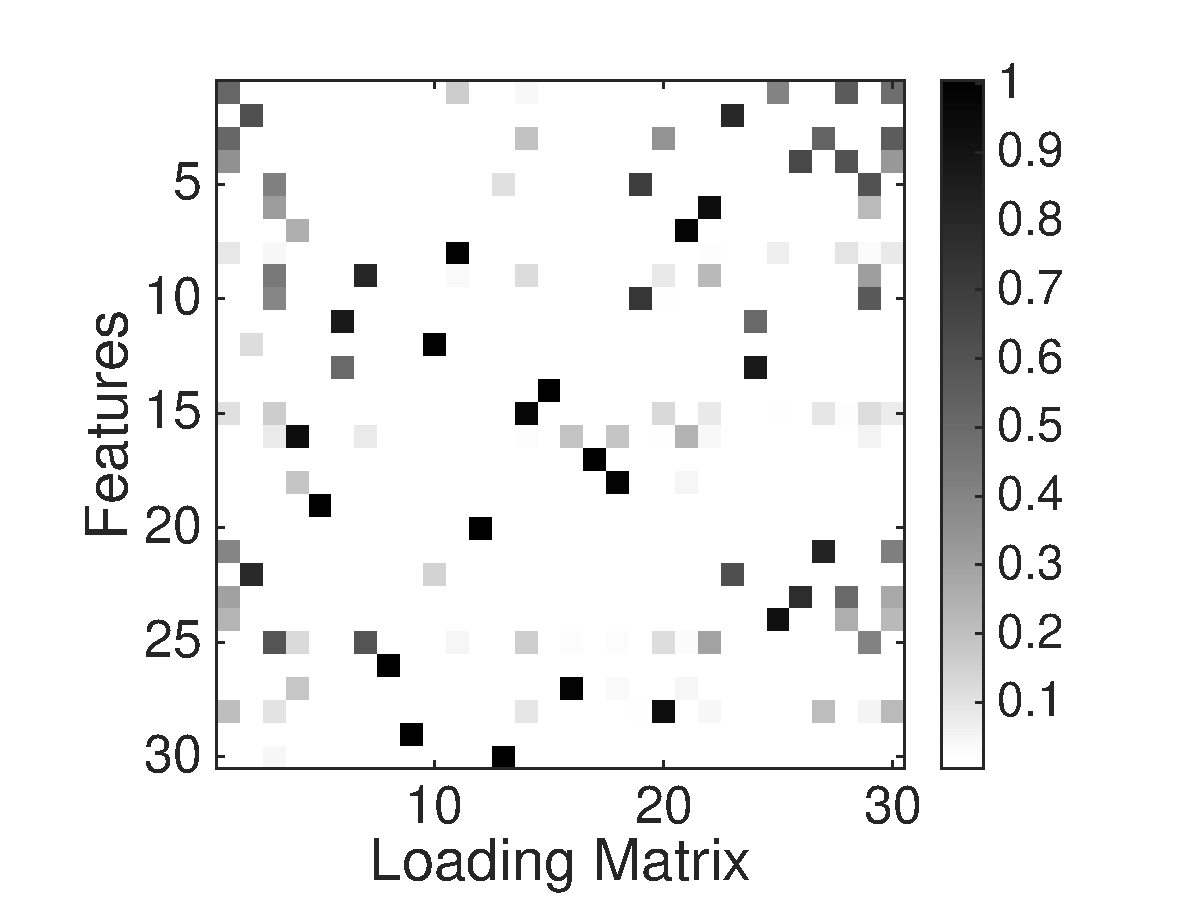
\includegraphics[width=35mm]{figure/new/Cancer-Components-ASPCA-F}}
    \subcaptionbox{}{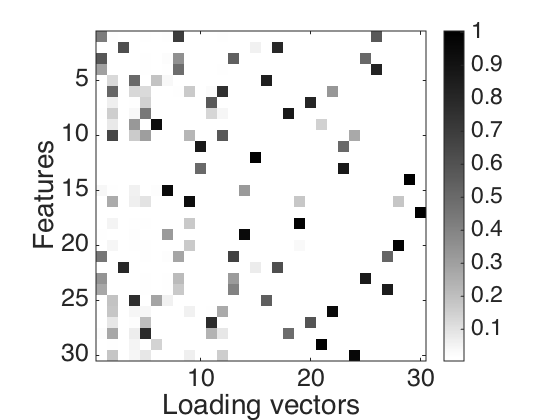
\includegraphics[width=35mm]{figure/new/Cancer-Components-ASPCA-B}}
    \subcaptionbox{}{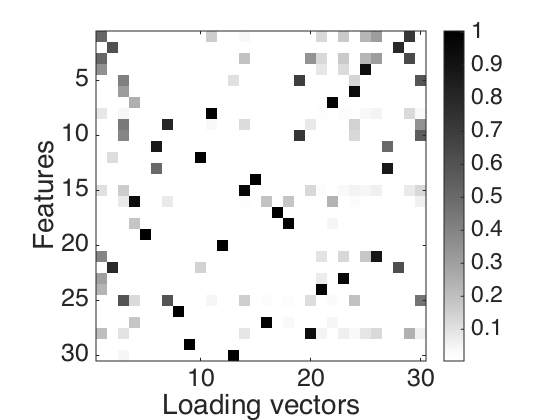
\includegraphics[width=35mm]{figure/new/Cancer-Components-ASPCA-FG}}
    \subcaptionbox{}{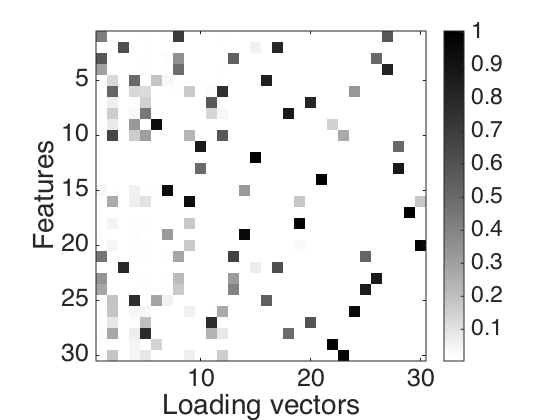
\includegraphics[width=35mm]{figure/new/Cancer-Components-ASPCA-BG}}
	\\
    \subcaptionbox{}{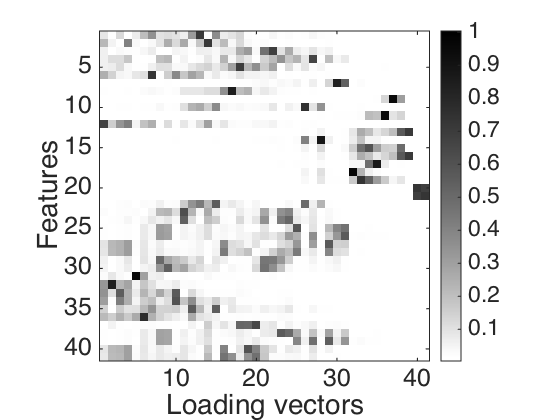
\includegraphics[width=35mm]{figure/new/KDD-Components-100-6-PCA}}
    \subcaptionbox{}{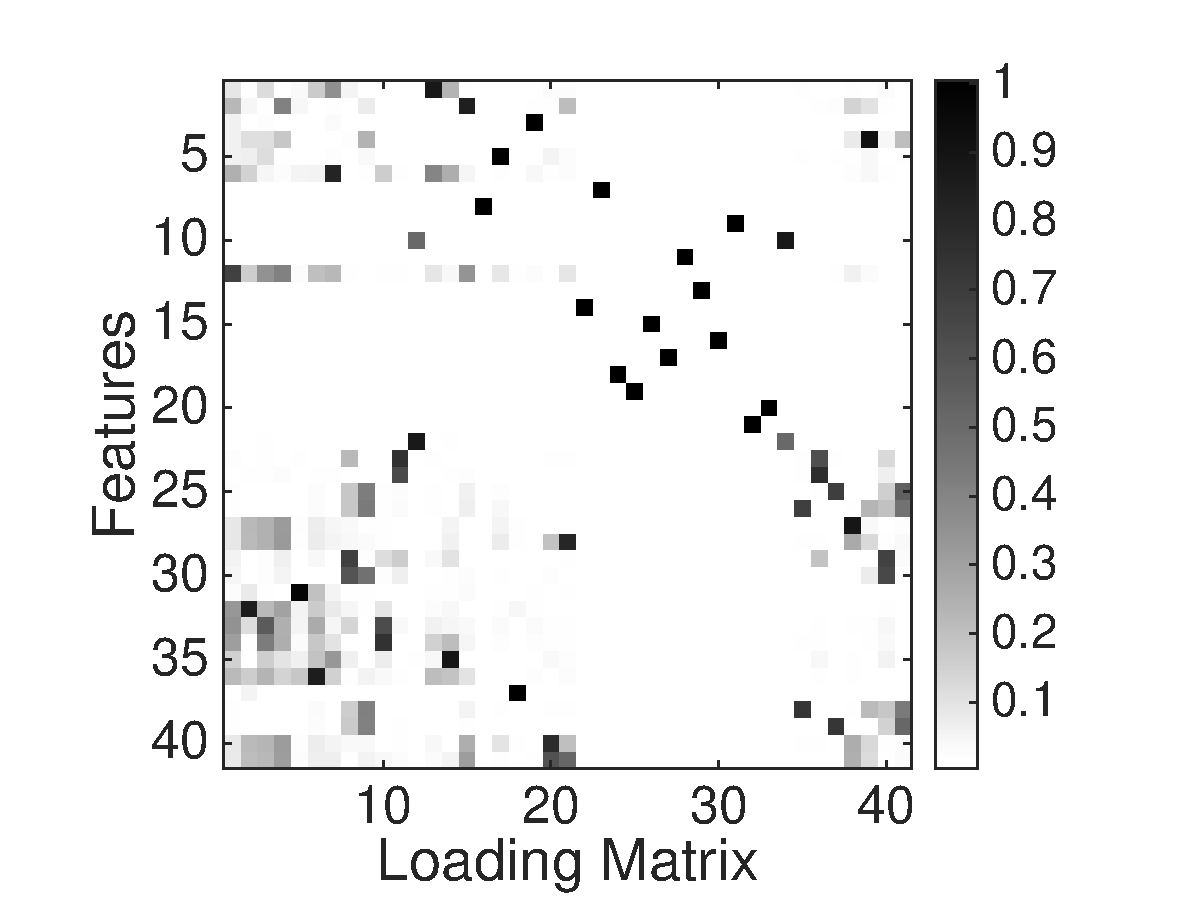
\includegraphics[width=35mm]{figure/new/KDD-Components-100-6-ASPCA-F}}
    \subcaptionbox{}{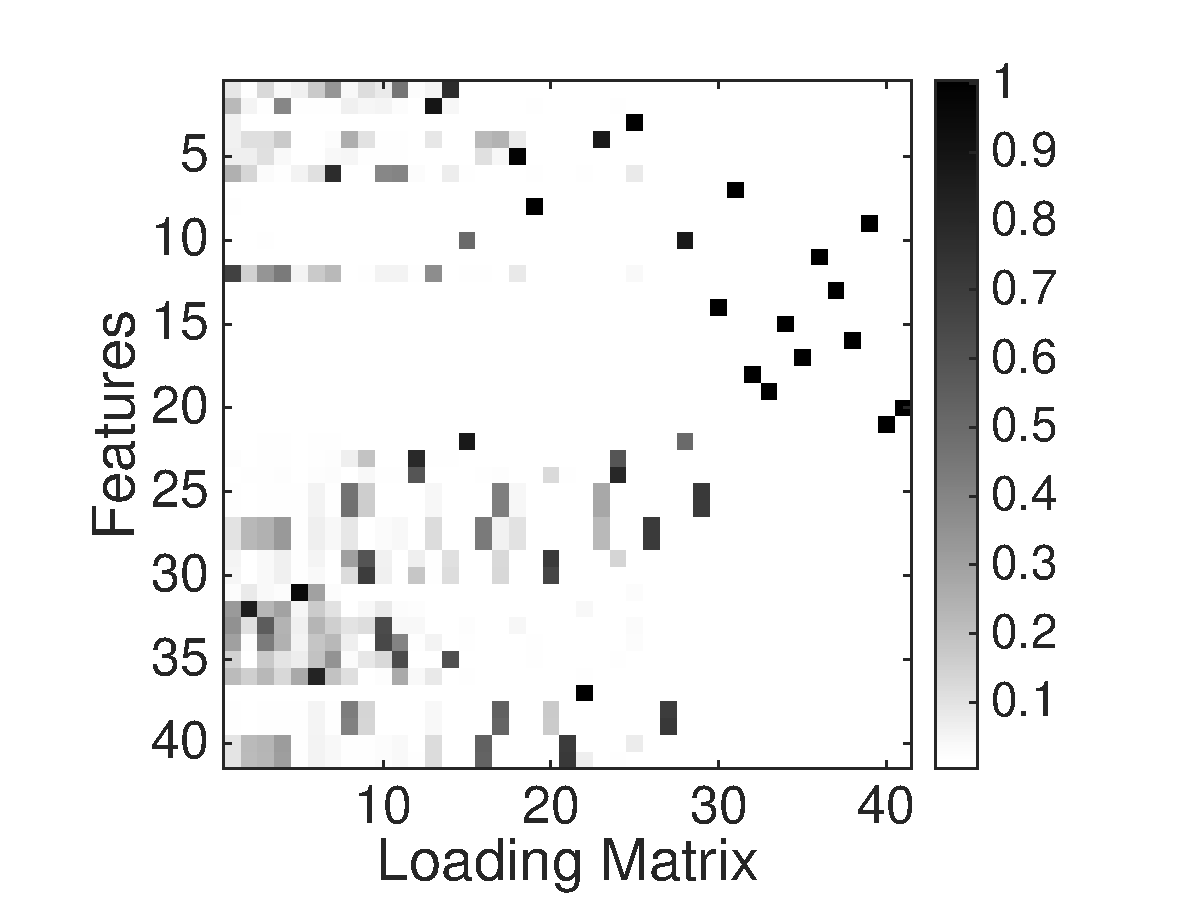
\includegraphics[width=35mm]{figure/new/KDD-Components-100-6-ASPCA-B}}
    \subcaptionbox{}{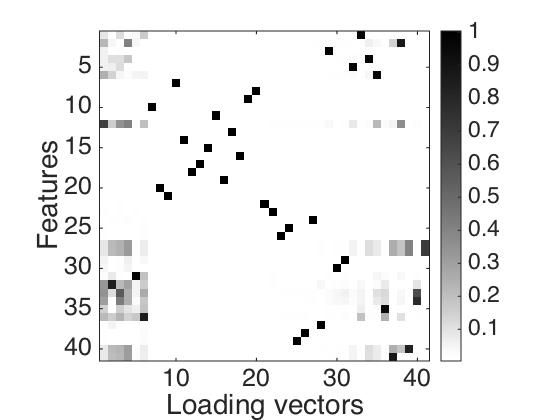
\includegraphics[width=35mm]{figure/new/KDD-Components-100-6-ASPCA-FG}}
    \subcaptionbox{}{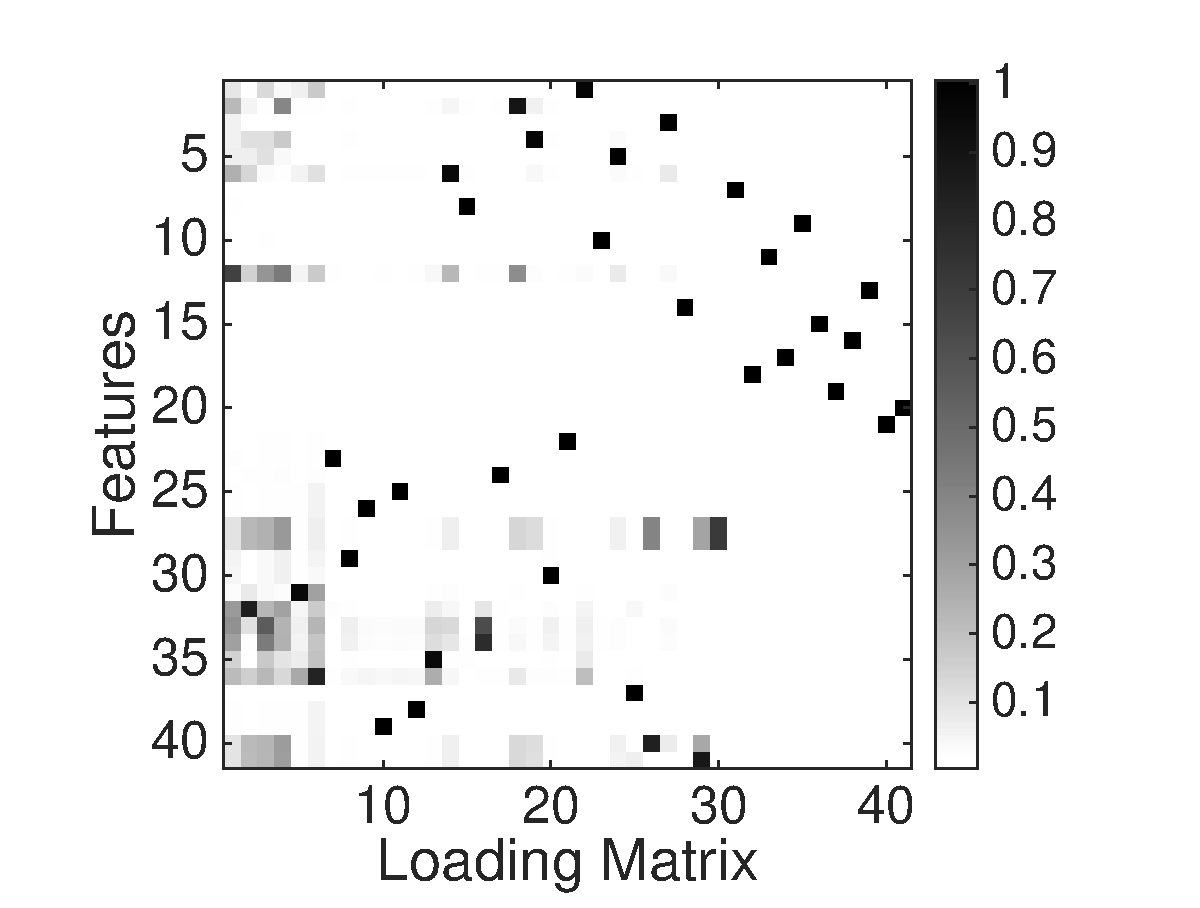
\includegraphics[width=35mm]{figure/new/KDD-Components-100-6-ASPCA-BG}}
\caption{Loading matrix of PCs of Breast-Cancer (Top) and KDD99 (Bottom) obtained by PCA, ASPCA-F, ASPCA-B, ASPCA-FG, and ASPCA-BG from left to right}
\label{fig:components}
\end{figure*}

\subsubsection{可解释性}

Now we evaluate the interpretation performance of the ASPCA-BG model, as it has the best sparsity performance. Since we want to see how true anomalies are interpreted by our model, we selected a threshold value on SPE to ensure most of the true anomalies are detected. We show the threshold values, false positive rates (FPR), and true positive rates (TPR) for all three datasets in Table~\ref{table:threshold}.

\begin{table}
\small
\centering
\caption{SPE Threshold}
\begin{tabular}{|l|l|l|l|}
\hline
              & SPE threshold & TPR    & FPR    \\ \hline
Synthetic     & 0.25          & 1      & 0      \\ \hline
Breast-Cancer & 0.1003  & 1      & 0.0476 \\ \hline
KDD99        & 0.5075      & 0.8516 & 0.0657 \\ \hline
\end{tabular}
\label{table:threshold}
\end{table}

{\bf Synthetic Data:}
The four abnormal PCs and the projection values of 15 anomalies on these PCs are shown in Table~\ref{table:components:synthetic} and Figure~\ref{fig:heatmap:synthetic}, respectively. As shown in Table~\ref{table:components:synthetic}, the first three PCs correspond to the rules of $D \approx C + A$, $A \approx B$,  and $F \approx 0$, respectively. The anomalies breaking these rules indeed have large projection values on the corresponding PCs. Thus, our ASPCA-BG model can not only identify the set of
features that are responsible for an anomaly, but also tell the cause of the anomaly, \i.e., breaking the rules indicated by the abnormal PCs.

JSPCA also successfully identified the relevant features $(A, B, D, F)$ as suggested in Figure~\ref{fig:loading matrix:synthetic}. However, it cannot tell the source of each individual anomaly. Unlike JSPCA, our ASPCA models make no assumptions on whether there are anomalies present in the dataset for model training. Keeping only normal data from the Synthetic dataset,  the ASPCA-BG model found four abnormal PCs with loading vectors $(0.31, 0.31, 0.64, 0.64, 0, 0, 0)^T$, $(-0.71,$  $0.71, 0, 0, 0, 0)^T$, $(0, 0, 0, 0, 0, 1, 0)^T$ , and $(0, 0, 0, 0, 0, 0, 1)^T$, which are very similar to the ones in Table~\ref{table:components:synthetic}. Using these abnormal PCs, we can successfully detect and interpret anomalies as well.

\begin{figure}
\centering
	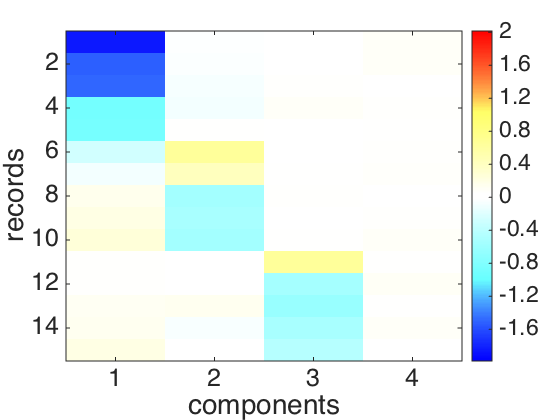
\includegraphics[width=42mm]{figure/new/Synthetic-heat-map}
\caption{Heatmap of projection values of anomalies on abnormal PCs for Synthetic Data}
\label{fig:heatmap:synthetic}
\end{figure}

\begin{table}
\centering
\caption{Components on Synthetic Data}
\label{table:components:synthetic}
\small
\begin{tabular}{|c|c|}
\hline
Index & Components \\ \hline
1 & 0.3099 A + 0.3122 B + 0.6370 C - 0.6330 D \\
2 & 0.7095 A - 0.7047 B\\
3 & 1 F\\
4 & 1 G\\
\hline
\end{tabular}
\end{table}

\begin{figure}
	\centering
	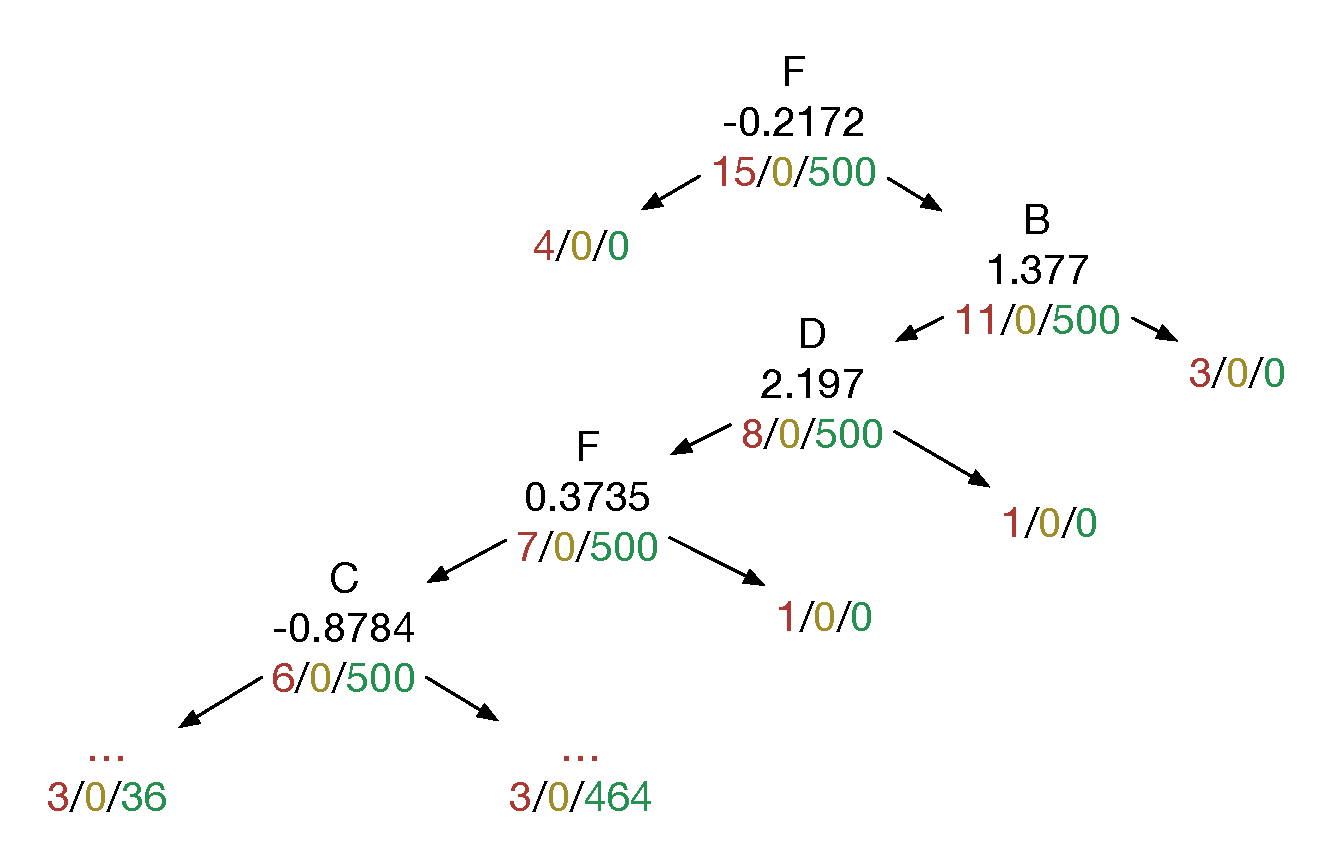
\includegraphics[width=60mm]{figure/new/Synthetic-DT}
	\caption{Decision tree on Synthetic Data}
\label{fig:dt:synthetic}
\end{figure}

The decision tree was shown in Figure~\ref{fig:dt:synthetic}, where on each node we showed the feature and its value used to partition the data, the number of true positives detected by ASPCA-BG in red, the number of false positives in yellow, and the number of normal data detected by ASPCA-BG in green. We can see that the decision tree model needs several rules to describe a group of anomalies which could be easily described by a clear linear combination and a threshold. In Figure~\ref{fig:dt:synthetic}, only the third type of anomalies, which has a large absolute value on F, is easy for the decision tree model to interpret.

{\bf Breast-Cancer:}
The projection values of 10 anomalies on the abnormal PCs obtained by ASPCA-BG for Breast-Cancer are shown in Figure~\ref{fig:heatmap:cancer}.  We can see that the malignant records have two patterns: the first four records have large projection values on the 2nd, 3rd, and 4th PCs, the rest records have large projection values on the first PC and moderate projection values on the 6th PC. We show these PCs in Table~\ref{table:breast_cancer}, where coefficients in PCs less than 0.1 were omitted.  The features appearing in the 1st and 6th PCs are \emph{area\_se}, \emph{area\_worst}, and \emph{radius\_worst}, which were reported previously by \cite{Wolberg1995792} as being effective for classifying malignant records.  Note that, \emph{area\_worst} actually has a quadratic relation with \emph{radius\_worst}, our model identified it as a linear relation, which is a good approximation in a small range of radius. The first four records, on the other hand, do not have large projection values on PCs related to \emph{area} features.  They were detected by PCs related to \emph{symmetry}, \emph{fractal dimension}, and \emph{compactness} features, which clearly indicates another type of malignant records.

\begin{figure}
\centering
	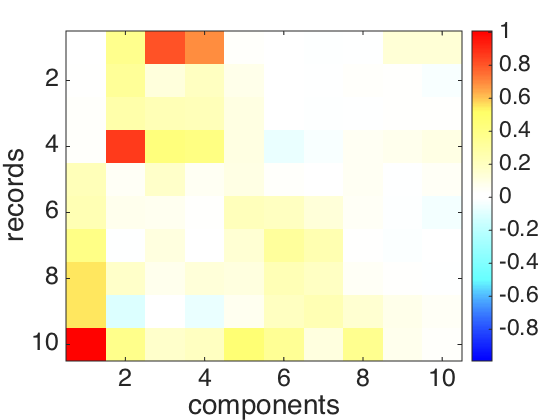
\includegraphics[width=50mm]{figure/new/Cancer-heat-map}
\caption{Heatmap of projection values of anomalies on abnormal PCs of Breast-Cancer}
\label{fig:heatmap:cancer}
\end{figure}

\begin{table}
\caption{Components on Breast-Cancer.}
\label{table:breast_cancer}
\small
\centering
\begin{tabular}{|c|c|}
\hline
Index & Components                                                                                                  \\ \hline
1     & 1 \emph{area\_se}                                                                                       \\ \hline
2     & 0.9894 \emph{symmetry\_worst}             \\ \hline
3     & \begin{tabular}[c]{@{}c@{}}0.9631 \emph{fractal\_dimension\_worst} \\ - 0.2693 \emph{fractal\_dimension\_mean}\end{tabular}                                                                                                 \\ \hline
4     & \begin{tabular}[c]{@{}c@{}}0.9445 \emph{compactness\_worst}\\  - 0.3286 \emph{compactness\_mean}\end{tabular}                                                                                              \\ \hline
%5     &  0.8631 perimeter\_worst - 0.5051 perimeter\_mean\\ \hline
6     & 0.8554 \emph{area\_worst} - 0.5180 \emph{radius\_worst}                                                                                \\ \hline
%7    & 0.8195 area\_mean - 0.5732 radius\_mean                                                                     \\ \hline
%8     & 0.8643 perimeter\_se - 0.5030 radius\_se                                                                    \\ \hline
%9     &     1 concavity\_se                                                        \\ \hline
%10     &    0.9841 fractal dimension\_se                                                                 \\ \hline
\end{tabular}
\end{table}

\begin{figure}
\centering
	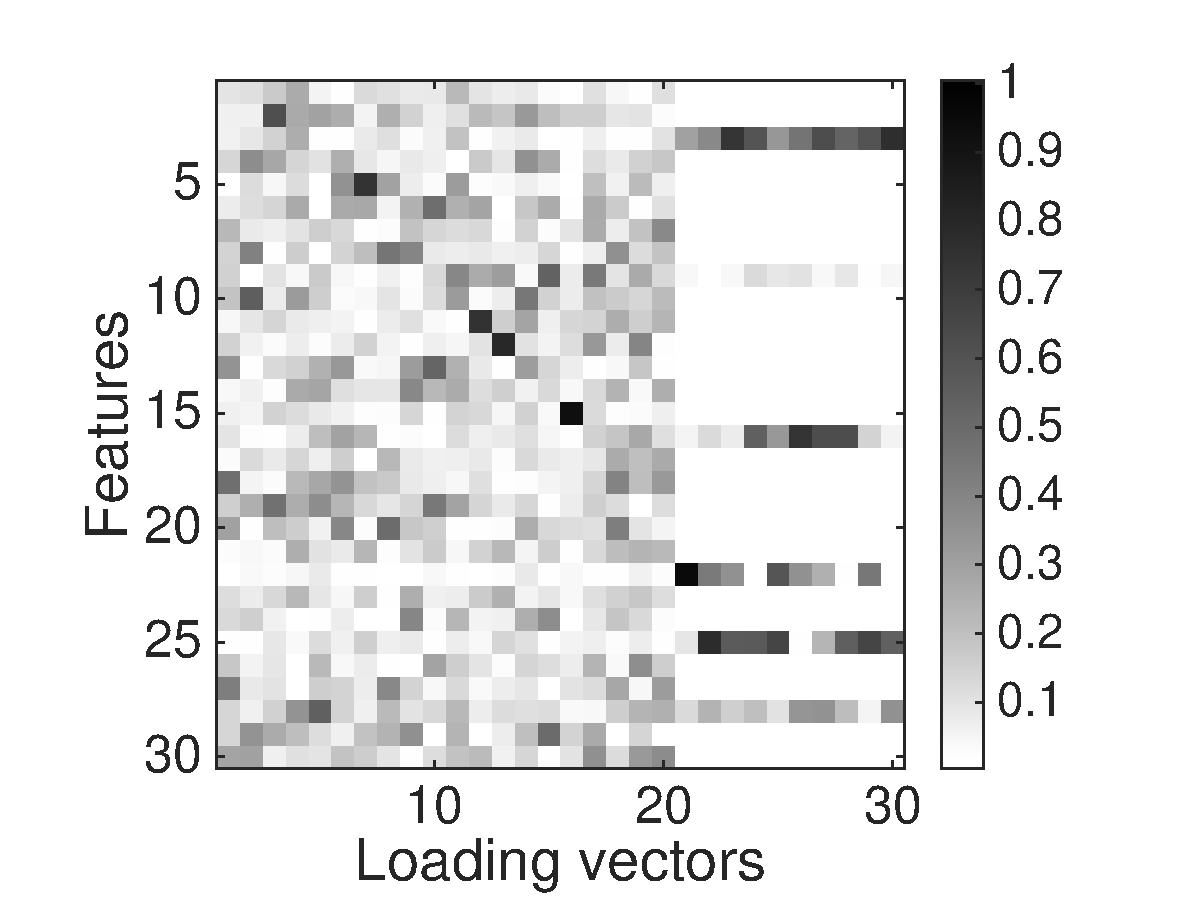
\includegraphics[width=42mm]{figure/Cancer-JSPCA-Components}
\caption{Loading matrix of abnormal PCs obtained by JSPCA on Breast-Cancer}
\label{fig:JSPCA:cancer}
\end{figure}

\begin{figure}
\centering
	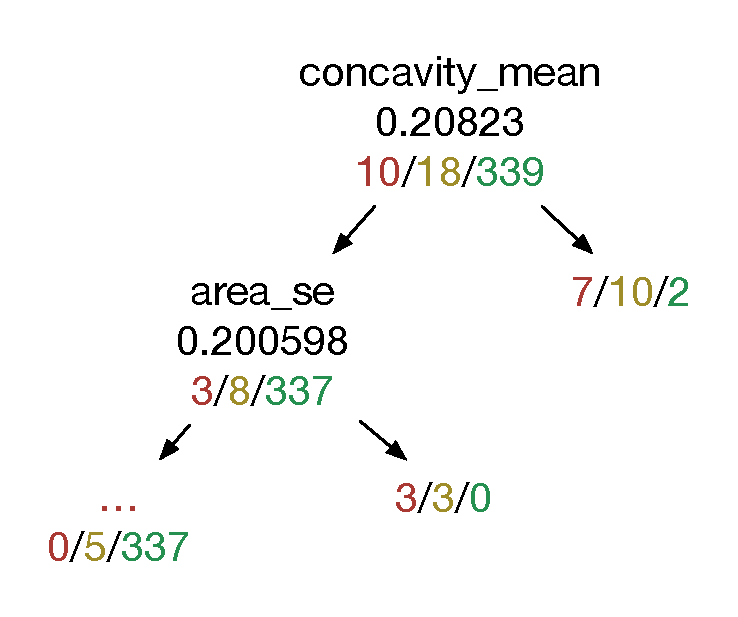
\includegraphics[width=40mm]{figure/new/Cancer-DT}
	\caption{Decision tree on Breast-Cancer}
         \label{fig:tree:cancer}
\end{figure}

The loading matrix of the abnormal PCs obtained by JSPCA on Breast-Cancer is shown in Figure~\ref{fig:JSPCA:cancer}. The relevent features are \emph{radius\_mean}, \emph{concavity\_mean}, \emph{area\_se}, \emph{fractal\_} \emph{dimension\_se}, \emph{perimeter\_worst}, and \emph{compactness\_worst}. As we can see, JSPCA cannot tell the different causes of individual anomalies.
The decision tree obtained on Breast-Cancer is shown in Figure~\ref{fig:tree:cancer}. Our ASPCA-BG model detected 10 true positives, 18 false positives, and 339 true negatives (shown on the root node in red, yellow, and green, respectively) with the chosen SPE threshold. The tree used \emph{concavity\_mean} to separate positive and negative samples. However, the attribute \emph{concavity\_mean} is orthogonal to the abnormal subspace obtained by our ASPCA-BG model, which means it is not the feature based on which our ASPCA-BG model detects anomalies. Hence, using decision trees to interpret results of a subspace-based model, such as ours, may lead to misleading interpretations.

{\bf KDD99:}
With the given SPE threshold, our ASPCA-BG model detected 4397 true positives on KDD99. Although our model is intended to analyze individual anomalies, we can also summarize interpretations of similar anomalies to make our discussion easier. We used a simple way to generate signatures on whether an anomaly has \emph{low} ($\leq -\sqrt{SPE threshold/2}$), or \emph{high} ($\geq \sqrt{SPE threshold/2}$) projection values on the set of abnormal PCs. Then anomalies were grouped according to their signatures, so that the components in the signature of each group is common for most of the anomalies in the group.

In Table~\ref{table:signatures on KDD}, we listed some major signatures found by the above method. Actually, for most of the cases, we can associate each signature group with an anomaly type quite well.  The two numbers listed for each anomaly type are the number of detected anomalies by our model and the number of total anomalies of this type, respectively. The two numbers listed for each signature group are the number of the anomalies of this type and the total number of anomalies in the group, respectively. Some anomaly types only have one main corresponding signature groups, whereas we identified three main signature groups for warezclient{[}R2L{]}. For the $i$th PC, $i$L and $i$H represent low and high projection values on it, respectively.  Finally, the components appeared in these signatures are shown in Table~\ref{table:components on KDD}.

\begin{table}
\small
\caption{Signatures on KDD99}
\label{table:signatures on KDD}
\centering
\begin{tabular}{|c|c|l|}
\hline
                                                                                         & \# in Type/              & Important       \\
Type                                                                                     & \# in Group              & Components      \\ \hline
\multirow{2}{*}{\begin{tabular}[c]{@{}c@{}}neptune{[}DoS{]}\\ 500/500\end{tabular}}      & \multirow{2}{*}{481/484} & 2L, 9H, 10H     \\
                                                                                         &                          & 11H, 12H, 14H   \\ \hline
\begin{tabular}[c]{@{}c@{}}smurf{[}DoS{]}\\ 493/500\end{tabular}                         & 472/472                  & 1H, 3L, 8H, 16H \\ \hline
\begin{tabular}[c]{@{}c@{}}teardrop{[}DoS{]}\\ 496/500\end{tabular}                      & 393/393                  & 18H             \\ \hline
\begin{tabular}[c]{@{}c@{}}satan{[}Probe{]}\\ 500/500\end{tabular}                       & 444/444                  & 2L, 3H, 6H, 8H  \\ \hline
\begin{tabular}[c]{@{}c@{}}portsweep{[}Probe{]}\\ 354/500\end{tabular}                  & 175/175                  & 6H, 7L          \\ \hline
\begin{tabular}[c]{@{}c@{}}ipsweep{[}Probe{]}\\ 217/500\end{tabular}                     & 104/109                  & 1H, 19H         \\ \hline
\multirow{3}{*}{\begin{tabular}[c]{@{}c@{}}warezclient{[}R2L{]}\\ 974/1020\end{tabular}} & 272/395                  & 15H, 20H        \\ \cline{2-3}
                                                                                         & 332/339                  & 4L, 5H, 6L      \\ \cline{2-3}
                                                                                         & 237/292                  & 4L, 5H          \\ \hline
\begin{tabular}[c]{@{}c@{}}guess-passwd{[}R2L{]}\\ 53/53\end{tabular}                    & 48/121                   & 4H, 5H          \\ \hline
\begin{tabular}[c]{@{}c@{}}buffer-overflow{[}U2R{]}\\ 30/30\end{tabular}                 & 7/7                      & 5H, 24H         \\ \hline
\end{tabular}
\end{table}

From Table~\ref{table:signatures on KDD}, we can see that the signatures for different anomaly types varied a lot, from which we often can find the components that are consistent with the nature of each anomaly type. For example, smurf[DoS] attacks are also known as popular form of DoS packet floods, which turn out to have high \emph{srv\_count} and \emph{count} values ({\it i.e.}, 16H and 8H). Teardrop[DoS] attacks try to break the host by sending mangled IP fragments, which led to high \emph{wrong\_fragment} values ({\it i.e.}, 18H).  We can see similar trends for Probe attacks too. For example, ipsweep[Probe] attacks sweep different hosts (IPs) to find cracks for hacking ({\it i.e.}, 19H), whereas portsweep[Probe] attacks try to visit different service ({\it i.e.}, 6H) and short connection duration ({\it i.e.}, 7L). Buffer overflow[U2R] attackers try to gain the root authority on the host, and 24H indicates that the user has logged into the server with root shell. Warezclient[R2L] attackers try to download files in forbidden directories from the FTP servers. Our interpretation is consistent with \cite{sabhnani2003kdd} as \emph{logged\_in} with low \emph{dst\_bytes} ({\it i.e.}, 4L), \emph{is\_guest\_login} ({\it i.e.}, 15H) and high \emph{hot} values ({\it i.e.}, 20H).

\begin{table}
\small
\caption{Components on KDD99}
\label{table:components on KDD}
\centering
	\begin{tabular}{|c|c|}
\hline
Index & Components                                                                                                                   \\ \hline
1     & 0.8906 \emph{protocol\_type} + 0.3658 \emph{logged\_in}                                                                                    \\ \hline
2     & 0.9949 \emph{same\_srv\_rate}                                                                                                       \\ \hline
3     & 0.9958 \emph{diff\_srv\_rate}                                                                                                       \\ \hline
4     & \begin{tabular}[c]{@{}c@{}}0.9520 \emph{dst\_bytes} \\ - 0.2222 \emph{logged\_in}\end{tabular}                                             \\ \hline
5     & \begin{tabular}[c]{@{}c@{}}0.7722 \emph{dst\_host\_same\_srv\_rate} \\ - 0.6286 \emph{dst\_host\_srv\_count}\end{tabular}                  \\ \hline
6     & \begin{tabular}[c]{@{}c@{}}0.9466 \emph{dst\_host\_diff\_srv\_rate}\end{tabular}       \\ \hline
7     & 0.9714 \emph{duration}                                                                                                              \\ \hline
8     & 0.9995 \emph{count}                                                                                                                 \\ \hline
9     & 0.9716 \emph{flag}                                                                                                                  \\ \hline
10    & 0.9984 \emph{dst\_host\_serror\_rate}                                                                                               \\ \hline
11    & 0.9981 \emph{srv\_serror\_rate}                                                                                                     \\ \hline
12    & 0.9981 \emph{serror\_rate}                                                                                                          \\ \hline
14    & 0.9985 \emph{dst\_host\_srv\_serror\_rate}                                                                                          \\ \hline
15    & 0.9997 \emph{is\_guest\_login}                                                                                                      \\ \hline
16    & 0.9994 \emph{srv\_count}                                                                                                            \\ \hline
18    & 0.9996 \emph{wrong\_fragment}                                                                                                       \\ \hline
19    & 0.9970 \emph{dst\_host\_srv\_diff\_host\_rate}                                                                                      \\ \hline
20    & 0.9999 \emph{hot}                                                                                                                   \\ \hline
24    & 1 \emph{root\_shell}                                                                                                                \\ \hline
	\end{tabular}
\end{table}


The results obtained by JSPCA are shown in Table~\ref{Table:KDD 99}. The selected features by JSPCA are more general and similar for all categories. Some of the important features for specific attacks are missing too, for instance, \emph{root\_shell} for User-2-Root[U2R] attacks and \emph{hot} and \emph{is\_guest\_login} for R2L attacks as mentioned in \cite{sabhnani2003kdd}.

We show the decision tree obtained on KDD99 in Figure~\ref{fig:tree:KDD}. The features captured by the decision tree are consistent with the components discovered by our ASPCA-BG model to a large extent. For example, low \emph{same\_srv\_rate} was chosen to detect neptune and satan DoS attackers, which is the same as using 2L in our model to detect the same attacks. Similarly, high \emph{protocol\_type} values ({\it i.e.}, using ICMP protocol) was chosen to detect ipsweep and smurf attackers (detected by 1H in our model). Low \emph{dst\_host\_srv\_count} with high \emph{hot} values is an important character of warezclient and guess-passed attacks  (identical to 5H and 20H in our model). An interesting observation on the decision tree in Figure~\ref{fig:tree:KDD} is that a node on the tree will stop splitting as soon as the samples in the node are mostly positive or negative ones. For example, the left child node of the root in Figure~\ref{fig:tree:KDD} stopped splitting with anomalies from different attack types, in which case, our model can provide more information on the differences of the these attack types.
\begin{figure}
\centering
	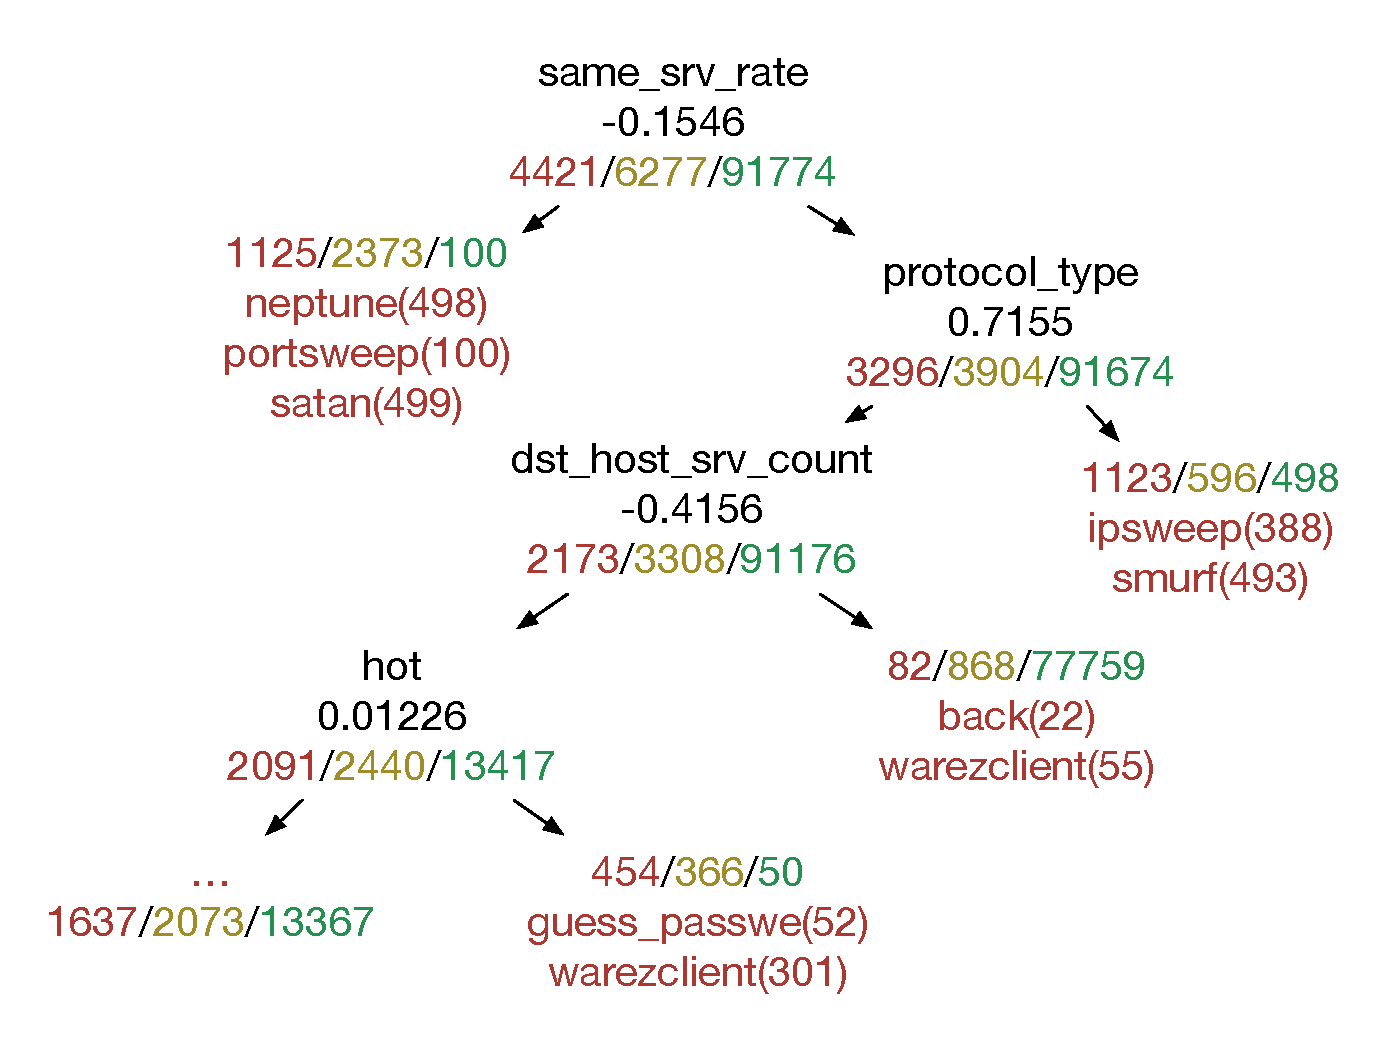
\includegraphics[width=70mm]{figure/new/KDD-DT}
	\caption{Decision tree on KDD99}
         \label{fig:tree:KDD}
\end{figure}


\subsection{Parameter Selection}
\label{sec:parameter}
Our ASPCA models has two parameters to select: the number of abnormal PCs and the coefficient $\lambda$ on sparsity. We know that PCA-based anomaly detection methods are sensitive to the number of PCs \cite{PCA-Sensitivity}. We plotted the detection accuracy (in terms of Area Under ROC Curve (AUC)) with different number of abnormal PCs on Breast-Cancer (with $\lambda=5$) and KDD99 ($\lambda=100$) in Figure~\ref{Figure:parameter:components}. We selected 20 normal PCs ({\it i.e.}, 10 abnormal PCs) for Breast-Cancer data and 6 normal PCs ({\it i.e.}, 35 abnormal PCs), for KDD99 data, to achieve the highest AUC values for our baseline method PCA, to make the comparisons on detection accuracy fair.

The coefficient $\lambda$ is a trade-off between the sparsity and the additional variance on components. With less additional variance, the variances on the whole detection space for various ASPCA models are closer to the one of PCA. We showed the variance, sparsity (valued by $||V||_{1,1}$) and AUC values obtained by varying the value of $\lambda$ on KDD99 and Breast-Cancer in Table~\ref{Table:parameter:lambada} for ASPCA-FG and ASPCA-BG. We can see that our models are not very sensitive to $\lambda$  in terms of AUC, and we selected $\lambda=5$ for Breast-Cancer, $\lambda=100$ for KDD99 for moderate sparsity and variance. The trends are similar for ASPCA-F and ASPCA-B, which were omitted due to space constraints. We selected the same $\lambda$ values for ASPCA-F and ASPCA-B, as in ASPCA-FG and ASPCA-BG, respectively.


\begin{figure}
\centering
\subcaptionbox{Breast-Cancer}
{
	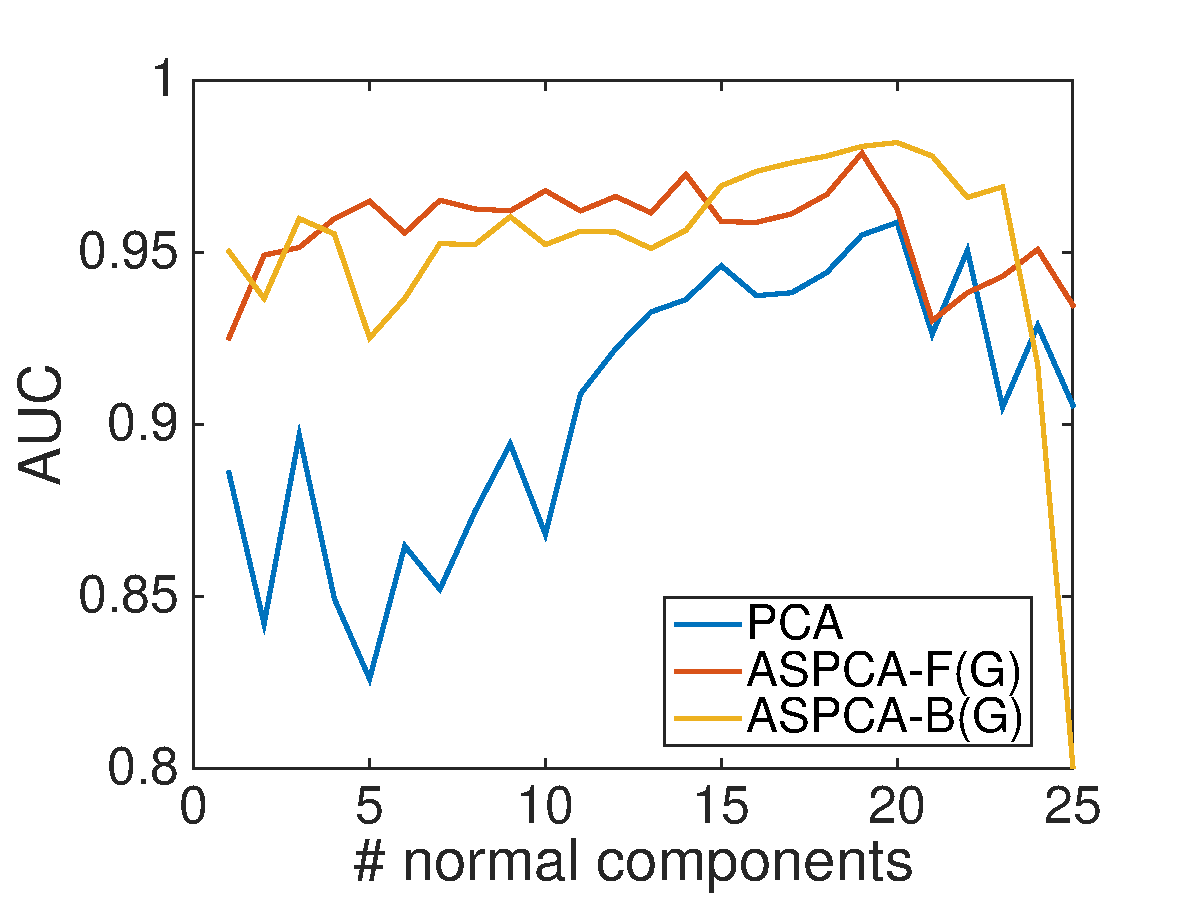
\includegraphics[width=40mm]{figure/new/Cancer-AUC-Components}
}
\subcaptionbox{KDD99}
{
	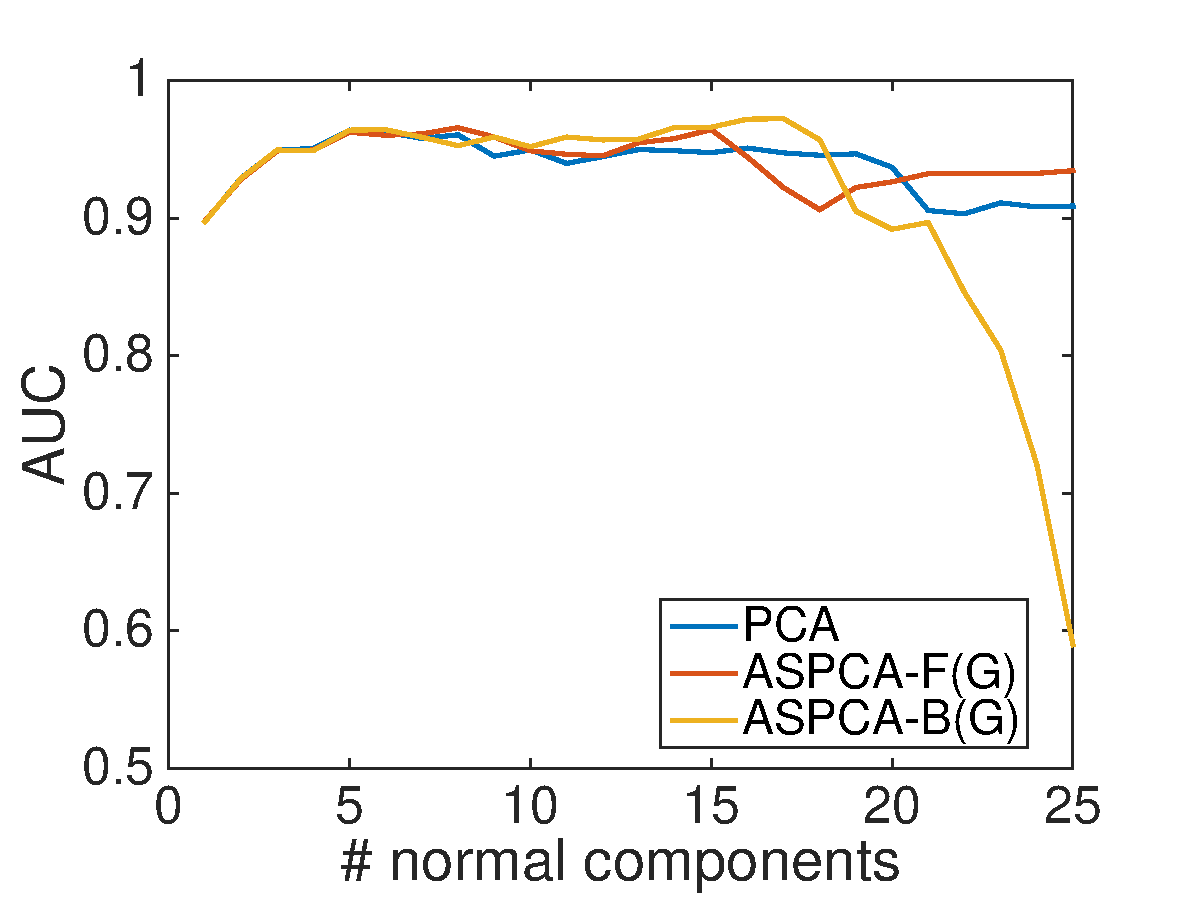
\includegraphics[width=40mm]{figure/new/KDD-AUC-Components}
}
\caption{Selection on the number of normal PCs}
\label{Figure:parameter:components}
\end{figure}


\begin{table*}
\centering
\caption{Selection on $\lambda$ for KDD99}

\begin{tabular}{|l|l|l|l|l|l|l|}
\hline
\multicolumn{1}{|l|}{} & \multicolumn{3}{c|}{ASPCA-FG}    & \multicolumn{3}{c|}{ASPCA-BG}    \\ \hline
$\lambda$ & $||V||_{1,1}$ & Variance & AUC   & $||V||_{1,1}$ & Variance & AUC   \\ \hline
0         & 97.33         & 21518    & 0.963 & 97.33         & 21518    & 0.963 \\
10        & 44.38         & 21524    & 0.963 & 44.59         & 21523    & 0.963 \\
50        & 43.52         & 21627    & 0.962 & 43.97         & 21589    & 0.964 \\
100       & 42.77         & 21873    & 0.960 & 43.04         & 21735    & 0.964 \\
500       & 41.04         & 23673    & 0.956 & 40.67         & 22997    & 0.967 \\ \hline
\end{tabular}
\end{table*}
\begin{table*}
\caption{Selection on $\lambda$ for Breast-Cancer}
\begin{tabular}{|l|l|l|l|l|l|l|}
\hline
\multicolumn{1}{|l|}{} & \multicolumn{3}{c|}{ASPCA-FG}    & \multicolumn{3}{c|}{ASPCA-BG}    \\ \hline
$\lambda$              & $||V||_{1,1}$ & Variance & AUC   & $||V||_{1,1}$ & Variance & AUC   \\ \hline
0                      & 34.23         & 1.2728   & 0.959 & 34.23         & 1.2728   & 0.959 \\
1                      & 26.68         & 14.2012  & 0.903 & 14.95         & 6.2777   & 0.950 \\
5                      & 16.50         & 20.8308  & 0.963 & 12.31         & 20.2968  & 0.982 \\
10                     & 12.81         & 30.8123  & 0.985 & 10            & 57.0009  & 0.966 \\
50                     & 10            & 57.0009  & 0.966 & 10            & 57.0009  & 0.966 \\ \hline
\end{tabular}
	\label{Table:parameter:lambada}

\end{table*}

\chapter{结论}

Traditional PCA-based anomaly detection models are not suitable for anomaly interpretation, limiting its usage in the domains where interpretation is essential.  In this paper, we found that the sparsity and orthogonality of the loading vectors are the keys to anomaly interpretation, and proposed an interpretable PCA-based anomaly detection model, the ASPCA model. We designed \emph{forward} and \emph{backward} ASPCA models and evaluated them on two real world datasets. Our model achieved similar or even better anomaly detection performance as the traditional PCA model, and provided meaningful interpretation for individual anomalies. Our future works will focus on three directions: 1) how to improve efficiency on high dimensional datasets; 2) how to extend our model to robust PCA for better detection performance; 3) how to extend our model to kernel PCA.


%%% 其它部分
\backmatter

%% 本科生要这几个索引,研究生不要。选择性留下。
% 插图索引
%% \listoffigures
% 表格索引
%% \listoftables
% 公式索引
%% \listofequations


%% 参考文献
% 注意:至少需要引用一篇参考文献,否则下面两行可能引起编译错误。
% 如果不需要参考文献,请将下面两行删除或注释掉。
\bibliographystyle{thuthesis}
\bibliography{ref/refs}


%% 致谢
\include{data/ack}

%% 附录
%% \begin{appendix}
%% \input{data/appendix01}
%% \end{appendix}

%% 个人简历
%% \include{data/resume}
\end{document}
